% ============================================================================
% Accessibility
% ============================================================================
\DocumentMetadata{
  lang = en-US, 
  pdfstandard = ua-2, 
  tagging = on, 
  tagging-setup = {math/setup=mathml-SE}
}

% ============================================================================
% Document Properties - used on title slide and PDF metadata fields
% ============================================================================
\def\PresTitle{Screw Threads and Thread Gauges}  % Required - top line of title slide
\def\PresSubtitle{Baker College Engineering}         % Optional - second line
\def\PresAuthor{Brad Peirson}               % Required - below dividing line
\def\PresInstitute{College of Information Technology and Engineering}       % Optional
\def\PresDate{}                             % Optional
\def\PresKeywords{}                         % Optional - used for hyperref

% Presentation Formatting
% ============================================================================
% ============================================================================
% Class Declaration
% ============================================================================
\documentclass[
        mode = handout,     % Projector = one bullet at a time, Handout = all
        font-size=14pt,     % Only accepts 9, 10, 12, 14, 17, 20
        pdfusetitle         % Pulls \title property from document
    ]
    {ltx-talk}              % ltx-talk class

% ============================================================================
% Custom Colors
% ============================================================================
\usepackage[table]{xcolor}
% Colors from the Baker College Style Guide
%\definecolor{BakerADARed}{RGB}{231, 0, 46}   % #e7002e Official ADA red-doesn't pass WCAG AAA for small text
\definecolor{BakerADARed}{RGB}{181, 0, 36}    % #b50024 Adjusted ADA red-passes WCAG AAA for small text
\definecolor{HoneyYellow}{RGB}{255, 196, 0}   % #ffc400
\definecolor{UpNorthGreen}{RGB}{114, 191, 68} % #72bf44
\definecolor{LakeBlue}{RGB}{134, 183, 227}    % #86b7e3
\definecolor{BakerADI}{RGB}{58, 98, 170}
\definecolor{BakerCIM}{RGB}{217, 35, 47}
\definecolor{BakerBlack}{RGB}{31, 34, 40}     % #1f2228
\definecolor{BakerWhite}{RGB}{255, 255, 255}
\definecolor{BakerRed}{RGB}{239, 0, 48}
\definecolor{Abbey}{RGB}{80, 82, 88}
\definecolor{RollingStone}{RGB}{121, 124, 126}
\definecolor{HitGray}{RGB}{165, 169, 172}
\definecolor{Iron1}{RGB}{201, 206, 209}
\definecolor{Iron}{RGB}{222, 225, 226}
\definecolor{BlackHaze1}{RGB}{237, 240, 240}
\definecolor{BlackHaze}{RGB}{245, 247, 247}

% ============================================================================
% Document Data
% ============================================================================
\title{\PresTitle}
\author{\PresAuthor}
\institute{\PresInstitute}
\date{\PresDate}

%Set up the hyperlink colors
\hypersetup{colorlinks,
    linkcolor=BakerBlack,
    urlcolor=BakerADARed,
    pdfauthor = {\PresAuthor},
    %pdftitle = {\PresentationTopic},   % Title is pulled directly
    pdfsubject = {\PresSubtitle},
    pdfkeywords = {\Keywords},
    pdfcreator = {LaTeX with hyperref package},
    pdfproducer = {LuaLaTeX}
    }

% Map your custom style guide colors to the progress bar aliases
\colorlet{pbcomplete}{BakerADARed}
\colorlet{pbincomplete}{Iron}

\usepackage[most]{tcolorbox}

% ============================================================================
% Footer Format
% ============================================================================
\EditInstance{footer}{std}{
  color         = Abbey,
  separator     = \hfill,
  element-order = {title, institute, framenumber},
  right-hspace  = 3mm,
  left-hspace   = 3mm,
}

% \DeclareInstance{footer}{empty}{
%   element-order = {}
% }

% ============================================================================
% Progress Bar Toggles & Helper Macros
% ============================================================================
\usepackage{xfp}        % Needed for floating point math
\newif\ifprogressbar    % Used to determine whether or not to show the bar
\progressbartrue        % Set the bar to true at the start

% Helper macro to automatically turn off the progress bar inside title/section frames
\newcommand{\makeblindframe}[1]{%
  \progressbarfalse
  #1%
  \progressbartrue
}

% ============================================================================
% Custom Page Formats
% ============================================================================
\let\oldmaketitle\maketitle         % Backup the original maketitle command
\let\oldsection\section             % Backup the original section command
\let\oldsubsection\subsection       % Backup the original subsection command

\makeatletter
\renewcommand{\maketitle}{%
\makeblindframe{%
  \disableglobalbackground
  \slidebackground{PresentationTitleGraphic_2048x1151}%
  \color{white}%
  %\UseInstance{footer}{wallpaper}
  \begin{frame}[wallpaper]
    \vspace*{1in}%
      \begin{tcolorbox}[
          enhanced,
          colback=black,       
          colframe=black,      
          opacityfill=0.25,       
          arc=6pt,                
          boxrule=0pt,            
          left=20pt, right=20pt,  
          top=20pt, bottom=20pt,
          width=0.80\textwidth,   
          halign=left             
      ]
          \color{white}%
          % Title (Always visible)
          {\large\bfseries\sffamily \@title}\\[0.5em]%
          
          % Conditional Subtitle
          \ifx\PresSubtitle\empty
          \else
            {\normalsize\sffamily \PresSubtitle}\\[0.5em]%
          \fi
          
          % High-contrast divider line
          {\color{white!80}\rule{0.3\textwidth}{0.8pt}}\\[0.5em]%
          
          % Author (Always visible)
          {\small\sffamily \@author}\\%
          
          % Conditional Institute
          \ifx\PresInstitute\empty
          \else
            {\small\sffamily \PresInstitute}\\%
          \fi
          
          % Conditional Date
          \ifx\PresDate\empty
          \else
            {\small\sffamily \@date}\\%
          \fi
      \end{tcolorbox}%
      \vfill     
  \end{frame}%
  \enableglobalbackground{BG}%
  \color{black}%
  %\UseInstance{footer}{std}
}%
}
\makeatother

% Create a variable container to hold the current section title
\newcommand{\currentsectiontitle}{}

% Redefine \section to take 1 argument (the title)
\renewcommand{\section}[1]{%
\makeblindframe{%
  \renewcommand{\currentsectiontitle}{#1}%
  \disableglobalbackground
  \slidebackground{PresentationSectionBackground_2048x1151}%
  \begin{frame}
    \vfill
    %\vspace*{0.625in}%
    \begin{tcolorbox}[
        enhanced,
        colback=black,       
        colframe=black,      
        opacityfill=0.25,       
        arc=6pt,                
        boxrule=0pt,            
        left=20pt, right=20pt,  
        top=20pt, bottom=20pt,
        width=0.80\textwidth,   
        halign=left             
    ]
        \color{white}%
        {\large\bfseries\sffamily #1}\\[0.5em]%   
    \end{tcolorbox}%
    \vfill 
  \end{frame}%
  \oldsection{#1}%
  \enableglobalbackground{BG}%

  % This will be used for an auto TOC at every section
  % Right now ltx-talk TOC is still in development
  % Once it comes a little further along this can be used
  % \begin{frame}
  %       \frametitle{Section Overview}
  %       \tableofcontents[sections=\thesection]
  %   \end{frame}%
}%
}

% Redefine \subsection to take 1 argument
\renewcommand{\subsection}[1]{%
\makeblindframe{%
  \disableglobalbackground
  \slidebackground{PresentationSectionBackground_2048x1151}%
  \begin{frame}
    \vfill
    %\vspace*{0.25in}% 
    \begin{tcolorbox}[
        enhanced,
        colback=black,       
        colframe=black,      
        opacityfill=0.25,       
        arc=6pt,                
        boxrule=0pt,            
        left=20pt, right=20pt,  
        top=20pt, bottom=20pt,
        width=0.80\textwidth,   
        halign=left             
    ]
        \color{white}%
        {\large\bfseries\sffamily\currentsectiontitle}\\[0.5em]%
        {\normalsize\sffamily #1}%
    \end{tcolorbox}%
    \vfill 
  \end{frame}%
  \oldsubsection{#1}%
  \enableglobalbackground{BG}%
}%
}

%Set the fonts to use NeueHaas Grotesk
\setsansfont{NHAASGROTESKTXPRO-}[
    Path=../NeueHaasGroteskFiles/,
    Scale=1.0,
    Extension = .ttf,
    UprightFont=*55Rg,
    BoldFont=*75Bd,
    ItalicFont=*56It,
    BoldItalicFont=*76BdIt
    ]

% Force the document default family to Sans-Serif
\renewcommand{\familydefault}{\sfdefault}

\usepackage{mathtools} % Load BEFORE unicode math settings
\setmathfont{Fira Math}[Scale=MatchLowercase] 

% 1. Turn global background ON
\newcommand{\enableglobalbackground}[1]{%
  \AddToHook{shipout/background}[mybg]{%
    \put(0, -\paperheight){%
      \includegraphics[width=\paperwidth, height=\paperheight, artifact]{#1}%
    }%
  }%
}

% 2. Turn global background OFF
\newcommand{\disableglobalbackground}{%
  \RemoveFromHook{shipout/background}[mybg]%
}

\newcommand{\slidebackground}[1]{%
  \AddToHookNext{shipout/background}{%
    \put(0, -\paperheight){%
      \includegraphics[width=\paperwidth, height=\paperheight, artifact]{#1}%
    }%
  }%
}

% --- GLOBAL BULLET OVERRIDES ---
\renewcommand{\labelitemi}{\color{BakerBlack}\Large\textbullet}
\renewcommand{\labelitemii}{\color{BakerBlack}\large\textbullet}
\renewcommand{\labelenumi}{\color{BakerBlack}\bfseries\arabic{enumi}.}
\renewcommand{\labelenumii}{\color{BakerBlack}\bfseries\alph{enumii})}

\AddToHook{begindocument/before}{%
  \EditInstance{item}{description}{
    label-format = \normalfont\bfseries\color{BakerADARed}#1
  }%
}

\AddToHook{begindocument/before}{%
  \EditInstance{item}{basic}{
    label-format = \color{BakerADARed}#1
  }%
}

% Global override for ltx-talk slide titles
\EditInstance{frametitle}{header}{
    font = \rule{0pt}{1.5cm}\bfseries\Large,
}

\EditInstance{header}{std}{
    font = \bfseries\huge,
    color = BakerBlack,
}

\AddToHook{env/block/begin}{%
  \colorlet{structure}{BakerADARed}%
}

\pretocmd{\tableofcontents}{\begin{minipage}{\textwidth} \linespread{1.4}}{}{}
\apptocmd{\tableofcontents}{\end{minipage}}{}{}

%Biber not functional in ltx-talk as of 2026-05-29
%Package that allows the creation of bibliographies
\usepackage[
    backend=biber,
    style=authoryear,
    sorting=none,
    %entryhead=false
    ]{biblatex}

%Load the bibliography file
\addbibresource{../../reference.bib}

\defbibheading{bibslide}{References}

\newcolumntype{L}[1]{>{\raggedright\let\newline\\\arraybackslash\hspace{0pt}}m{#1}}
\newcolumntype{C}[1]{>{\centering\let\newline\\\arraybackslash\hspace{0pt}}m{#1}}
\newcolumntype{R}[1]{>{\raggedleft\let\newline\\\arraybackslash\hspace{0pt}}m{#1}}

%All of the graphics are in a seperate folder, this makes it so the folder doesn't have to be repeated every time
\graphicspath{
  {../assets/images}
  {../assets/diagrams}
  {../assets/plots}
}

\makeatletter
% New counter to hold the custom "max frames" for the progress bar
\newcommand{\pb@maxtotal}{1}

% Read the custom total from the .aux file if it exists
\AtBeginDocument{%
  \ifdefined\pb@storedtotal
    \let\pb@maxtotal\pb@storedtotal
  \else
    % Fallback to standard total if our custom hook hasn't run yet
    \edef\pb@maxtotal{\@totalframes}%
  \fi
}

% Custom Appendix command that caps the progress bar and turns it off
\newcommand{\talkappendix}{%
  % 1. Write the CURRENT frame number to the .aux file as the progress total
  \immediate\write\@auxout{\string\gdef\string\pb@storedtotal{\@framenumber}}%
  % 2. Turn off the progress bar for all subsequent appendix slides
  \progressbarfalse
}
\makeatother

% ============================================================================
% Progress Bar Logic 
% ============================================================================
\makeatletter               
\AddToHook{shipout/background}{%
  \ifprogressbar
    % Read ltx-talk's internal frame counter safely
    \edef\currentframe{\@framenumber}%
    \edef\totalframes{\pb@maxtotal}% Use our custom max total instead
    
    % Fallback checks: If the document hasn't fully compiled yet, default to 1
    \ifx\currentframe\empty\def\currentframe{1}\fi
    \ifx\totalframes\empty\def\totalframes{1}\fi
    
    % Draw the progress bar if we have a valid total frame count
    \ifnum\totalframes>1\relax
      % Compute fraction width: (current - 1) / (total - 1)
      \edef\pbfraction{\fpeval{(\currentframe - 1) / (\totalframes - 1)}}%
      
      % Guard rails to prevent the bar from overshooting 100% on a first compile
      \ifdim\pbfraction pt>1pt\def\pbfraction{1}\fi 
      
      \edef\completewidth{\fpeval{\pbfraction * \paperwidth}}%
      \edef\incompletewidth{\fpeval{\paperwidth - \completewidth}}%
      
      % Render full-width progress bar at the top edge
      \put(0cm, -0.1cm){%
        \color{pbcomplete}\rule{\completewidth pt}{2pt}%
        \color{pbincomplete}\rule{\incompletewidth pt}{2pt}%
      }%
    \fi
  \fi
}
\makeatother

% 1. Globally shrink all caption components right as the caption engine fires
\AddToHook{cmd/@makecaption/before}{\footnotesize}

% 2. Declare and assign a blank plug to the kernel's caption label socket
\NewSocketPlug{caption/label}{nolabel}{}
\AssignSocketPlug{caption/label}{nolabel}

\usepackage{adjustbox}

\usepackage{amssymb}
\usepackage{amsmath}

\usepackage{animate}

\usepackage{calc} % Optional, but helpful for layout

\usepackage{multirow}

\usepackage{textcomp}

\usepackage[americanvoltages]{circuitikz}
\usepackage{pgfplots}
\usepackage{pgf-pie}

\usetikzlibrary{
    intersections, 
    fillbetween,
    patterns,
    decorations.pathreplacing,
    decorations.pathmorphing,
    decorations.text,
    decorations.markings,
    arrows.meta,
    arrows,
    shapes,
    shapes.geometric,
    shadows,
    calligraphy,
    backgrounds,
    intersections,
    calc,
    math,
    positioning,
    svg.path,
    shadows,
    shadows.blur
    }

\pgfplotsset{compat=1.18}

\pgfdeclarelayer{ft}
\pgfdeclarelayer{bg}
\pgfsetlayers{bg, main, ft}

% Usage: \hexpic[]{height}{Alt text}{Attribution}{image path}
\newcommand{\hexpic}[5][]{%
  \begin{figure}
    \centering
    \begin{tikzpicture}[
      baseline=(hex.base),      
      every shadow/.style={
        shadow opacity=70
        }
      ]
      \node (hex) [
        draw=white, 
        minimum size=#2, 
        regular polygon, 
        regular polygon sides=6, 
        rotate=90,
        blur shadow
      ] {};
      \begin{scope}
        \clip (hex.corner 1) -- (hex.corner 2) -- (hex.corner 3) -- 
              (hex.corner 4) -- (hex.corner 5) -- (hex.corner 6) -- cycle;
        \node at (hex.center) [#1] {
          \includegraphics[height=#2, alt={#3}]{#5}
        };
      \end{scope}
    \end{tikzpicture}

    \vspace{0.5em}
    {\tiny #4\par}
  \end{figure}  
}

% Usage: \shadowpic[]{width}{Alt text}{Attribution}{image path}
\newcommand{\shadowpic}[5][]{%
  \begin{figure}
    \centering
    \begin{tikzpicture}
      [every shadow/.style={
        shadow opacity=70
        }
      ]
      \node (image) [
        inner sep=0,
        blur shadow
      ] {\includegraphics[width=#2, alt={#3}]{#5}};
    \end{tikzpicture}

    \vspace{0.5em}
    {\tiny #4\par}
  \end{figure}
}

\tikzset{middlearrow/.style={
        decoration={markings, 
        mark= at position 0.5 with {\arrow{#1}},
        },
        postaction={decorate}
    }
}

% Usage: \tikztodo[width]{height}{description/notes}
\newcommand{\tikztodo}[3][0.8\textwidth]{%
  \begin{center}
    \fbox{%
      \parbox[c][#2][c]{#1}{%
        \centering
        \textbf{\textcolor{red}{TODO: TikZ Diagram}}\\[0.5em]
        \small #3%
      }%
    }%
  \end{center}%
}

% Macro: \drawrails{<number_of_1cm_segments>}
\newcommand{\drawrails}[1]{
  % Calculate total depth: 1 cm per segment
  \pgfmathsetmacro{\railheight}{-1 * #1}
  
  % L1 Rail (x = 0)
  \draw[thick] (0, 0) -- (0, \railheight cm);
    
  % L2 Rail (x = 15)
  \draw[thick] (15, 0) -- (15, \railheight cm);
}

\newcommand{\ccwplus}{%
  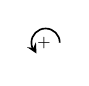
\begin{tikzpicture}[baseline=(char.base)]
    \node(char) at (0,0) {\(\scriptscriptstyle +\)};
    \draw[->, >=stealth, semithick] (0.2,0) arc (0:230:0.18cm);
  \end{tikzpicture}%
}

%====================================================================================
% Timer Ladder Symbol - Could be used for TON, TOF, RTO....
%====================================================================================
\tikzset{
    TON/.pic={

        \draw[
          BakerBlack
        ]
        (0,0)
        -- ++(0,0.375)
        -- ++(3.5,0)
        coordinate[pos=0.5](-TOP)
        -- ++(0,-1.75)
        coordinate[pos=3/14](-OUT)
        coordinate[pos=0.5](-EN1)
        coordinate[pos=0.875](-DN1)
        -- ++(-3.5,0)        
        -- (0,0)
        coordinate(-IN);

        \node[
          text=BakerBlack,
          font=\bfseries,
          anchor=east
        ](pre)
        at ($(-TOP)-(0,1.75em)$)
        {{\small PRE:}};

        \node[
          text=BakerBlack,
          font=\bfseries,
          anchor=east
        ](acc)
        at ($(pre.east)-(0,1em)$)
        {{\small ACC:}};

        \coordinate (-PRE) at (pre.east); % For the preset value
        \coordinate (-ACC) at (acc.east);

        \draw[
            BakerBlack
        ]
        (-EN1)
        -- ++(0.5,0)
        coordinate(-EN2)
        node[
            text=BakerBlack,
            anchor=west
        ]
        {{\small EN}};

        \draw[
            BakerBlack
        ]
        (-DN1)
        -- ++(0.5,0)
        coordinate(-DN2)
        node[
            text=BakerBlack,
            anchor=west
        ]
        {{\small DN}};

    }
}

%====================================================================================
% Oval ladder symbol, good for ONS, RES, etc.
%====================================================================================
\tikzset{
    ONS/.pic={

        \draw[
          BakerBlack
        ]
        (0,0)
        coordinate(-IN)
        -- ++(0.75,0)
        node[
          draw=BakerBlack, 
          text=BakerBlack, 
          font=\small, 
          minimum width=1.5cm, 
          minimum height=0.75cm, 
          anchor=west, 
          rounded corners=0.25cm
          ](ons){};
        
        \draw[BakerBlack] (ons.east) -- ++(0.75,0) coordinate(-OUT);

        \coordinate(-INS) at (ons.center);
        \coordinate(-VAR) at (ons.north); 
    }
}

%====================================================================================
% Source A, Source B, Dest box
%====================================================================================
\tikzset{
    SrcDest/.pic={
      
        \draw[
          BakerBlack
        ]
        (0,0)
        coordinate(-IN)
        -- ++(0,0.375)
        -- ++(5,0)
        coordinate[pos=0.5](-TOP)
        -- ++(0,-3.25)
        coordinate[pos=3/26](-OUT)
        -- ++(-5,0)
        -- (0,0)
        coordinate(l1);

        \node[
          text=BakerBlack,
          font=\bfseries,
          anchor=west
        ](srcA)
        at (l1)
        {{\small Src A:}};

        \node[
          text=BakerBlack,
          font=\bfseries,
          anchor=west
        ](srcB)
        at ($(l1)-(0,2em)$)
        {{\small Src B:}};

        \node[
          text=BakerBlack,
          font=\bfseries,
          anchor=west
        ](dest)
        at ($(srcB.west)-(0,2em)$)
        {{\small Dest:}};

        \coordinate(-SRCA) at (srcA.east);
        \coordinate(-AVAL) at ($(srcA.east)-(0,1em)$);
        \coordinate(-SRCB) at (srcB.east);
        \coordinate(-BVAL) at ($(srcB.east)-(0,1em)$);
        \coordinate(-DEST) at ($(-BVAL)-(0,1em)$);
        \coordinate(-DVAL) at ($(-DEST)-(0,1em)$);
    }
}

%====================================================================================
% Source A, Source B box
%====================================================================================
\tikzset{
    SrcAB/.pic={
      
        \draw[
          BakerBlack
        ]
        (0,0)
        coordinate(-IN)
        -- ++(0,0.375)
        -- ++(4,0)
        coordinate[pos=0.5](-TOP)
        -- ++(0,-2.25)
        coordinate[pos=1/6](-OUT)
        -- ++(-4,0)
        -- (0,0)
        coordinate(l1);

        \node[
          text=BakerBlack,
          font=\bfseries,
          anchor=west
        ](srcA)
        at (l1)
        {{\small Src A:}};

        \node[
          text=BakerBlack,
          font=\bfseries,
          anchor=west
        ](srcB)
        at ($(l1)-(0,2em)$)
        {{\small Src B:}};

        \coordinate(-SRCA) at (srcA.east);
        \coordinate(-AVAL) at ($(srcA.east)-(0,1em)$);
        \coordinate(-SRCB) at (srcB.east);
        \coordinate(-BVAL) at ($(srcB.east)-(0,1em)$);
    }
}

%====================================================================================
% LIMIT instruction
%====================================================================================
\tikzset{
    Limit/.pic={
      
        \draw[
          BakerBlack
        ]
        (0,0)
        coordinate(-IN)
        -- ++(0,0.375)
        -- ++(4,0)
        coordinate[pos=0.5](-TOP)
        -- ++(0,-3.25)
        coordinate[pos=3/26](-OUT)
        -- ++(-4,0)
        -- (0,0)
        coordinate(l1);

        \node[
          text=BakerBlack,
          font=\bfseries,
          anchor=west
        ](srcA)
        at (l1)
        {{\small Low:}};

        \node[
          text=BakerBlack,
          font=\bfseries,
          anchor=west
        ](srcB)
        at ($(l1)-(0,2em)$)
        {{\small Test:}};

        \node[
          text=BakerBlack,
          font=\bfseries,
          anchor=west
        ](dest)
        at ($(srcB.west)-(0,2em)$)
        {{\small High:}};

        \coordinate(-LO) at (srcA.east);
        \coordinate(-LOV) at ($(srcA.east)-(0,1em)$);
        \coordinate(-TEST) at (srcB.east);
        \coordinate(-TESTV) at ($(srcB.east)-(0,1em)$);
        \coordinate(-HI) at ($(-TESTV)-(0,1em)$);
        \coordinate(-HIV) at ($(-HI)-(0,1em)$);
    }
}

%====================================================================================
% Source Destination box
%====================================================================================
\tikzset{
    SrcSingle/.pic={
      
        \draw[
          BakerBlack
        ]
        (0,0)
        coordinate(-IN)
        -- ++(0,0.375)
        -- ++(6,0)
        coordinate[pos=0.5](-TOP)
        -- ++(0,-2.25)
        coordinate[pos=1/6](-OUT)
        -- ++(-6,0)
        -- (0,0)
        coordinate(l1);

        \node[
          text=BakerBlack,
          font=\bfseries,
          anchor=west
        ](srcA)
        at (l1)
        {{\small Source:}};

        \node[
          text=BakerBlack,
          font=\bfseries,
          anchor=east
        ](srcB)
        at ($(srcA.east)-(0,2em)$)
        {{\small Dest:}};

        \coordinate(-SRC) at (srcA.east);
        \coordinate(-SRCV) at ($(srcA.east)-(0,1em)$);
        \coordinate(-DEST) at (srcB.east);
        \coordinate(-DESTV) at ($(srcB.east)-(0,1em)$);
    }
}

%====================================================================================
% Compute Box
%====================================================================================
\tikzset{
    CPT/.pic={
      
        \draw[
          BakerBlack
        ]
        (0,0)
        coordinate(-IN)
        -- ++(0,0.375)
        -- ++(8.5,0)
        coordinate[pos=0.5](-TOP)
        -- ++(0,-1.75)
        coordinate[pos=3/14](-OUT)
        -- ++(-8.5,0)
        -- (0,0)
        coordinate(l1);

        \node[
          text=BakerBlack,
          font=\bfseries,
          anchor=west
        ](srcA)
        at (l1)
        {{\small Source:}};

        \node[
          text=BakerBlack,
          font=\bfseries,
          anchor=east
        ](srcB)
        at ($(srcA.east)-(0,2em)$)
        {{\small Exp:}};

        \coordinate(-DEST) at (srcA.east);
        \coordinate(-DESTV) at ($(srcA.east)-(0,1em)$);
        \coordinate(-EXP) at (srcB.east);
        \coordinate(-EXPV) at ($(srcB.east)-(0,1em)$);
    }
}

% ============================================================================
% Document Content
% ============================================================================
\begin{document}

\maketitle              % Redefined in the preamble to generate a full frame

\begin{frame}
    \frametitle{Agenda}
    \begingroup
        % Tighten the spacing between paragraphs/TOC lines
        \setlength{\parskip}{0.3em} 
        
        % Optionally tighten the line spacing within an entry
        %\baselineskip=1.2em 
        
        \setcounter{tocdepth}{1} % Show only sections
    \tableofcontents
    \setcounter{tocdepth}{2} % Reset back to default so subsections are tracked
    \endgroup
\end{frame}

\begin{frame}
    \frametitle{Simple Machines}

    \shadowpic[]{0.375\linewidth}{A line art illustration grid displaying the six simple machines in separate panels with text labels below each. The top row shows a person using a lever to pry a large rock, a water well with a crank representing a wheel and axle, and a pulley hoisting a heavy box. The bottom row shows a person rolling a barrel up an inclined plane, a wedge driven into a tree stump, and screw jacks lifting a heavy beam.}{\textbf{Attribution:} Foster, Ellsworth D., ed; Hughes, James L. (James Laughlin), Public domain, via \href{https://commons.wikimedia.org/wiki/File:Six_simple_machines.png}{Wikimedia Commons}}{Six_simple_machines}

    \vspace{0.5em}
    \centering
    {\footnotesize The screw is one of six \emph{simple machines}--the basic machines on which all other machines are based.\par}
\end{frame}

\begin{frame}
	\frametitle{The Archimedes Screw}
    \begin{columns}
        \begin{column}{0.48\linewidth}
            \begin{itemize}[<+- | alert@+>]
                \item One of the oldest and simplest machines 
                \item Dates back to at least Archimedes ($\sim$220 B.C.) who used it to pump water
                \item Some historians believe the Egyptians were using it earlier
            \end{itemize}
        \end{column}
        \begin{column}{0.48\linewidth}
            \shadowpic[]{0.625\linewidth}{An Archimedes screw water pump mechanism installed along stone steps at a outdoor park playground, leading down into a small pond of murky green water with wooden play structures including a pirate ship visible in the background.}{\textbf{Attribution:} Cavaliere grande, \href{https://creativecommons.org/licenses/by-sa/4.0}{CC BY-SA 4.0}, via \href{https://commons.wikimedia.org/wiki/File:Archimedes\%27_screw_Pleinfeld.jpg}{Wikimedia Commons}}{Archimedes'_screw_Pleinfeld}
        \end{column}
    \end{columns}
\end{frame}

\begin{frame}
	\frametitle{Further Development}
    \begin{columns}
        \begin{column}{0.48\linewidth}
            \begin{itemize}[<+- | alert@+>]
                \item Screw press used for squeezing grapes and olives
                \item DaVinci used screws in many inventions--invented the buttress thread
            \end{itemize}
        \end{column}
        \begin{column}{0.48\linewidth}
            \hexpic[]{0.875\linewidth}{A close-up view of a traditional wooden basket wine press featuring vertical wooden staves bound by a dark metal band with locking pins. Atop the basket rests a stacked wooden pressing block assembly driven downward by a heavy central threaded metal screw with a horizontal turning lever.}{\textbf{Attribution:} Alexander Baxevanis, \href{https://creativecommons.org/licenses/by/2.0}{CC BY 2.0}, via \href{https://commons.wikimedia.org/wiki/File:Grape_Press_At_Blandy\%27s_Wine_Lodge,_Funchal,_Madeira.jpg}{Wikimedia Commons}, cropped from original}{Grape_Press_At_Blandy's_Wine_Lodge,_Funchal,_Madeira}
        \end{column}
    \end{columns}
\end{frame}

\section{Thread Standards}

\begin{frame}
    \frametitle{The Wild West of Screw Threads}

    \shadowpic[]{0.375\linewidth}{Two views of a post-medieval copper alloy rein guide or check rein hook, showing front and back views against a white background with a centimeter scale ruler along the bottom and left edges. Each piece features an ornamental spiral-curved hook set above a collar and a threaded stem designed for mounting.}{\textbf{Attribution:} The Portable Antiquities Scheme, \href{https://creativecommons.org/licenses/by/2.0}{CC BY 2.0}, via \href{https://commons.wikimedia.org/wiki/File:Post_Medieval_copper_alloy_rein_guide_or_check_rein_hook_(FindID_502856).jpg}{Wikimedia Commons}}{Post_Medieval_copper_alloy_rein_guide_or_check_rein_hook_(FindID_502856)}

    \vspace{0.5em}
    \centering
    {\footnotesize For a \emph{very} long time craftsmen would use whatever thread shape suited them--as on these post medieval hooks.\par}
\end{frame}

\begin{frame}
    \frametitle{The Whitworth Thread}

    \shadowpic[]{0.875\linewidth}{A metal thread pitch gauge stamped with WHITWORTH 55 degrees and MADE IN GERMANY, featuring two sets of fan-folded metal blades with precision-toothed edges extending from opposite ends of a central holder.}{\textbf{Attribution:} Cccefalon, \href{https://creativecommons.org/licenses/by-sa/3.0}{CC BY-SA 3.0}, via \href{https://commons.wikimedia.org/wiki/File:Thread_pitch_gauge_Whitworth_and_metric.jpg}{Wikimedia Commons}}{Thread_pitch_gauge_Whitworth_and_metric}

    \vspace{0.5em}
    \centering
    {\footnotesize In 1841 Sir Joseph Whitworth created the first standard \emph{thread form}.\par}
\end{frame}

\begin{frame}
    \frametitle{Standardization of Screw Threads (1 of 2)}

    \shadowpic[]{0.75\linewidth}{Eight dark metal hex head bolts arranged in a semi-circular fan on a plain background, displaying various thread pitch and standard options. From left to right, they include Metric M12 left-handed thread, Metric M12 standard, Metric Fine M12x1.5, Metric Fine M12x1.25, Unified Fine UNF 1/2 inch, Unified Coarse UNC 1/2 inch, British Standard Whitworth BSW 1/2 inch, and British Standard Fine BSF 1/2 inch.}{\textbf{Attribution:} Christoph Roser at AllAboutLean.com, \href{https://creativecommons.org/licenses/by-sa/4.0}{CC BY-SA 4.0}, via \href{https://commons.wikimedia.org/wiki/File:Different_Thread_Types_Update.jpg}{Wikimedia Commons}}{Different_Thread_Types_Update}

    \vspace{0.5em}
    \centering
    {\footnotesize Today, the metric world is on the ISO thread standard.\par}
\end{frame}

\begin{frame}
    \frametitle{Standardization of Screw Threads (2 of 2)}

    \shadowpic[]{0.75\linewidth}{Eight dark metal hex head bolts arranged in a semi-circular fan on a plain background, displaying various thread pitch and standard options. From left to right, they include Metric M12 left-handed thread, Metric M12 standard, Metric Fine M12x1.5, Metric Fine M12x1.25, Unified Fine UNF 1/2 inch, Unified Coarse UNC 1/2 inch, British Standard Whitworth BSW 1/2 inch, and British Standard Fine BSF 1/2 inch.}{\textbf{Attribution:} Christoph Roser at AllAboutLean.com, \href{https://creativecommons.org/licenses/by-sa/4.0}{CC BY-SA 4.0}, via \href{https://commons.wikimedia.org/wiki/File:Different_Thread_Types_Update.jpg}{Wikimedia Commons}}{Different_Thread_Types_Update}

    \vspace{0.5em}
    \centering
    {\footnotesize The U.S. standardized on American Standard threads for a long time. That standard was eventually supplemented by the Unified Standard thread. In 1949, American Standard was officially obsoleted and was wholly replaced by Unified Standard.\par}
\end{frame}

\begin{frame}
    \frametitle{The Various Thread Standards}

    \shadowpic[]{0.75\linewidth}{Eight dark metal hex head bolts arranged in a semi-circular fan on a plain background, displaying various thread pitch and standard options. From left to right, they include Metric M12 left-handed thread, Metric M12 standard, Metric Fine M12x1.5, Metric Fine M12x1.25, Unified Fine UNF 1/2 inch, Unified Coarse UNC 1/2 inch, British Standard Whitworth BSW 1/2 inch, and British Standard Fine BSF 1/2 inch.}{\textbf{Attribution:} Christoph Roser at AllAboutLean.com, \href{https://creativecommons.org/licenses/by-sa/4.0}{CC BY-SA 4.0}, via \href{https://commons.wikimedia.org/wiki/File:Different_Thread_Types_Update.jpg}{Wikimedia Commons}}{Different_Thread_Types_Update}

    \vspace{0.5em}
    \centering
    {\footnotesize Left to right: M12, 40mm LH -- M12, 40 mm -- M12x1.5, 40mm -- M12x1.25, 40mm -- UNF 1/2-20x1.5 -- UNC 1/2-13x1.5 -- BSW 1/2-12x1.5 -- BSF 1/2-16x1.5\par}
\end{frame}

\section{Thread Types}

\begin{frame}
	\frametitle{Types of Threads (1 of 2)}

    \shadowpic[]{\linewidth}{A technical diagram illustrating seven cross-sectional screw thread profiles labeled lowercase a through g. Profile a shows a sharp V-thread with a 60-degree angle. Profile b shows a standard American V-thread with flat crests and roots at a 60-degree angle. Profile c shows a Whitworth thread with rounded crests and roots at a 55-degree angle. Profile d shows a square thread profile. Profile e shows an Acme thread profile with a 29-degree angle. Profile f shows a buttress thread profile with a flat top and a 45-degree angled flank. Profile g shows a knuckle thread profile with fully rounded crests and roots. Each profile includes geometric dimension labels for pitch p and thread height H.}{\textbf{Attribution:} Carl Lars Svenson, Public domain, via \href{https://commons.wikimedia.org/wiki/File:Screw_thread_forms.png}{Wikimedia Commons}}{Screw_thread_forms}

    \vspace{0.5em}
    \centering
    {\footnotesize Left to right: V-thread -- American National Thread -- Whitworth -- Square -- Acme -- Buttress -- Knuckle\par}
\end{frame}

\begin{frame}
	\frametitle{Types of Threads (2 of 2)}

    \shadowpic[]{\linewidth}{A technical diagram illustrating seven cross-sectional screw thread profiles labeled lowercase a through g. Profile a shows a sharp V-thread with a 60-degree angle. Profile b shows a standard American V-thread with flat crests and roots at a 60-degree angle. Profile c shows a Whitworth thread with rounded crests and roots at a 55-degree angle. Profile d shows a square thread profile. Profile e shows an Acme thread profile with a 29-degree angle. Profile f shows a buttress thread profile with a flat top and a 45-degree angled flank. Profile g shows a knuckle thread profile with fully rounded crests and roots. Each profile includes geometric dimension labels for pitch p and thread height H.}{\textbf{Attribution:} Carl Lars Svenson, Public domain, via \href{https://commons.wikimedia.org/wiki/File:Screw_thread_forms.png}{Wikimedia Commons}}{Screw_thread_forms}

    \vspace{0.5em}
    \centering
    {\footnotesize Threads all serve the same basic purpose: as they rotate they (or what they're attached to) moves linearly. While they all serve that same purpose, not all types of threads are good at, or even capable of, the same jobs.\par}
\end{frame}

\begin{frame}
	\frametitle{V Threads}

    \begin{columns}
        \begin{column}{0.48\linewidth}
            \begin{itemize}[<+- | alert@+>]
                \item Early attempt at a standardized form
                \item Basic 60\textdegree ``V'' shape
            \end{itemize}
        \end{column}
        \begin{column}{0.48\linewidth}
            \begin{figure}
                \centering
                \resizebox{\linewidth}{!}{
                    \begin{circuitikz}[
        american, 
        >={Latex[length=5mm, width=2mm]},
        alt={}
    ]

    \draw[
        BakerBlack,
        ultra thick
    ]
    (0,0)
    coordinate(O)
    -- (60:2)
    coordinate(p1)
    -- ++(-60:2)
    -- ++(60:2)
    coordinate(p2)
    -- ++(-60:2)
    -- ++(60:2)
    coordinate(p3)
    -- ++(-60:2)
    coordinate(b3)
    -- ++(60:2)
    coordinate(p4)
    -- ++(-60:2)
    -- ++(0,-1)
    coordinate(bot)
    -- (bot -| O)
    -- (0,0);

    \draw[
        BakerADARed,
        shorten <=0.25cm
    ]
    (p1)
    -- ++(0,1)
    coordinate[midway](pd1);

    \draw[
        BakerADARed,
        shorten <=0.25cm
    ]
    (p2)
    -- ++(0,1)
    coordinate[midway](pd2);

    \draw[
        BakerADARed,
        <->
    ]
    (pd1)
    -- (pd2)
    node[
        midway,
        above
    ]{P};

    \draw[
        BakerADARed,
        shorten <=0.25cm
    ]
    (p3)
    -- ++(120:1)
    coordinate[midway](a1);

    \draw[
        BakerADARed,
        shorten <=0.25cm
    ]
    (p4)
    -- ++(60:1)
    coordinate[midway](a2);

    \draw[
        BakerADARed,
        <->
    ]
    (a1)
    arc(120:60:2.5)
    node[
        midway,
        above
    ]{60\textdegree};

    \draw[
        BakerADARed,
        shorten <=0.25cm
    ]
    (b3)
    -- ++(2.5,0)
    coordinate(h1)
    -- ++(1,0);

    \draw[
        BakerADARed,
        shorten <=0.25cm
    ]
    (p4)
    -- (p4 -| h1)
    coordinate(h2)
    -- ++(1,0);

    \draw[
        BakerADARed,
        <->
    ]
    (h1)
    -- (h2)
    node[
        midway,
        right
    ]
    {$H=0.866P$};


\end{circuitikz}
                }
            \end{figure}
        \end{column}
    \end{columns}
\end{frame}

\begin{frame}
	\frametitle{American National}

    \begin{columns}
        \begin{column}{0.48\linewidth}
            \begin{itemize}[<+- | alert@+>]
                \item Standard US thread before Unified
                \item Same basic standard as V thread and Unified Standard
                \item General fastening
            \end{itemize}
        \end{column}
        \begin{column}{0.48\linewidth}
            \begin{figure}
                \centering
                \resizebox{\linewidth}{!}{
                    \begin{circuitikz}[
        american, 
        >={Latex[length=5mm, width=2mm]},
        alt={A technical geometric diagram of a standard metric or Unified V-thread profile showing truncated triangular teeth drawn with a solid thick outline over a dashed V-point reference grid. Dimension lines label the pitch between crests as P, the thread height as H equals 0.6495P, the flat root width as P over 8, and an arc measurement indicating a 60 degree thread angle between flanks.}
    ]

    \draw[
        LakeBlue,
        thin,
        dashed
    ]
    (0,0)
    coordinate(O)
    -- (60:2)
    coordinate(p1)
    coordinate[pos=0.875](p11)
    -- ++(-60:2)
    coordinate(b1)
    coordinate[pos=0.125](p12)
    coordinate[pos=0.875](b11)
    -- ++(60:2)
    coordinate[pos=0.125](b12)
    coordinate[pos=0.875](p21)
    coordinate(p2)
    -- ++(-60:2)
    coordinate(b2)
    coordinate[pos=0.125](p22)
    coordinate[pos=0.875](b21)
    -- ++(60:2)
    coordinate(p3)
    coordinate[pos=0.125](b22)
    coordinate[pos=0.875](p31)
    -- ++(-60:2)
    coordinate[pos=0.125](p32)
    coordinate[pos=0.875](b31)
    coordinate(b3)
    -- ++(60:2)
    coordinate[pos=0.125](b32)
    coordinate[pos=0.875](p41)
    coordinate(p4)
    -- ++(-60:2)
    coordinate[pos=0.125](p42)
    coordinate[pos=0.875](b41);

    \draw[
        BakerBlack,
        ultra thick
    ]
    (O)
    -- (p11)
    -- (p12)
    -- (b11)
    -- (b12)
    -- (p21)
    -- (p22)
    -- (b21)
    -- (b22)
    -- (p31)
    -- (p32)
    -- (b31)
    -- (b32)
    -- (p41)
    -- (p42)
    -- (b41)
    -- ++(0,-1)
    coordinate(bot)
    -- (bot -| O)
    -- (0,0);

    \draw[
        BakerADARed,
        shorten <=0.25cm
    ]
    (p1)
    -- ++(0,1)
    coordinate[midway](pd1);

    \draw[
        BakerADARed,
        shorten <=0.25cm
    ]
    (p2)
    -- ++(0,1)
    coordinate[midway](pd2);

    \draw[
        BakerADARed,
        <->
    ]
    (pd1)
    -- (pd2)
    node[
        midway,
        above
    ]{P};

    \draw[
        BakerADARed,
        shorten <=0.25cm
    ]
    (p3)
    -- ++(120:1)
    coordinate[midway](a1);

    \draw[
        BakerADARed,
        shorten <=0.25cm
    ]
    (p4)
    -- ++(60:1)
    coordinate[midway](a2);

    \draw[
        BakerADARed,
        <->
    ]
    (a1)
    arc(120:60:2.5)
    node[
        midway,
        above
    ]{60\textdegree};

    \draw[
        BakerADARed,
        shorten <=0.25cm
    ]
    (b32)
    -- ++(2.5,0)
    coordinate(h1)
    -- ++(1,0);

    \draw[
        BakerADARed,
        shorten <=0.25cm
    ]
    (p42)
    -- (p42 -| h1)
    coordinate(h2)
    -- ++(1,0);

    \draw[
        BakerADARed,
        <->
    ]
    (h1)
    -- (h2)
    node[
        midway,
        right
    ]
    {$H=0.6495P$};

    \draw[
        BakerADARed,
        shorten <=0.25cm
    ]
    (b12)
    -- ++(1,0)
    coordinate(root1)
    -- ++(0.5,0)
    coordinate(rootRef);

    \draw[
        BakerADARed,
        shorten <=0.25cm
    ]
    (b1)
    -- (b1 -| root1)
    coordinate(root2)
    -- (b1 -| rootRef);

    \draw[
        BakerADARed,
        <-
    ]
    (root1)
    -- ++(0,1);

    \draw[
        BakerADARed,
        <-
    ]
    (root2)
    -- ++(0,-1.5)
    node[
        right
    ]
    {$\frac{P}{8}$};



\end{circuitikz}
                }
            \end{figure}
        \end{column}
    \end{columns}
\end{frame}

\begin{frame}
	\frametitle{Acme Thread}

    \begin{columns}
        \begin{column}{0.48\linewidth}
            \begin{itemize}[<+- | alert@+>]
                \item Thicker threads than most other designs
                \item Used strictly for linear motion
            \end{itemize}
        \end{column}
        \begin{column}{0.48\linewidth}
            \begin{figure}
                \centering
                \resizebox{\linewidth}{!}{
                    \begin{circuitikz}[
        american, 
        >={Latex[length=5mm, width=2mm]},
        alt={A technical geometric diagram of an Acme screw thread profile showing trapezoidal thread teeth drawn with a solid thick outline over a dashed reference grid. Horizontal dimension lines mark the pitch labeled P between crests and the thread height labeled 0.5P, while an arc measurement indicates a 29 degree included angle between adjacent thread flanks.}
    ]

    \draw[
        LakeBlue,
        thin,
        dashed
    ]
    (0,0)
    coordinate(O)
    -- (75.5:4)
    coordinate(p1)
    coordinate[pos=0.625](p11)
    -- ++(-75.5:4)
    coordinate(b1)
    coordinate[pos=0.375](p12)
    coordinate[pos=0.625](b11)
    -- ++(75.5:4)
    coordinate[pos=0.375](b12)
    coordinate[pos=0.625](p21)
    coordinate(p2)
    -- ++(-75.5:4)
    coordinate(b2)
    coordinate[pos=0.375](p22)
    coordinate[pos=0.625](b21)
    -- ++(75.5:4)
    coordinate(p3)
    coordinate[pos=0.375](b22)
    coordinate[pos=0.625](p31)
    -- ++(-75.5:4)
    coordinate[pos=0.375](p32)
    coordinate[pos=0.625](b31)
    coordinate(b3)
    -- ++(75.5:4)
    coordinate[pos=0.375](b32)
    coordinate[pos=0.625](p41)
    coordinate(p4)
    -- ++(-75.5:4)
    coordinate[pos=0.375](p42)
    coordinate[pos=0.625](b41);

    \draw[
        BakerBlack,
        ultra thick
    ]
    (O)
    -- (p11)
    -- (p12)
    -- (b11)
    -- (b12)
    -- (p21)
    -- (p22)
    -- (b21)
    -- (b22)
    -- (p31)
    -- (p32)
    -- (b31)
    -- (b32)
    -- (p41)
    -- (p42)
    -- (b41)
    -- (b41 |- O)
    % coordinate(bot)
    % -- (bot -| O)
    -- (0,0);

    \draw[
        BakerADARed,
        shorten <=0.25cm
    ]
    (p1)
    -- ++(0,1)
    coordinate[midway](pd1);

    \draw[
        BakerADARed,
        shorten <=0.25cm
    ]
    (p2)
    -- ++(0,1)
    coordinate[midway](pd2);

    \draw[
        BakerADARed,
        <->
    ]
    (pd1)
    -- (pd2)
    node[
        midway,
        above
    ]{P};

    \draw[
        BakerADARed,
        shorten <=0.25cm
    ]
    (p3)
    -- ++(104.5:1)
    coordinate[midway](a1);

    \draw[
        BakerADARed,
        shorten <=0.25cm
    ]
    (p4)
    -- ++(75.5:1)
    coordinate[midway](a2);

    \draw[
        BakerADARed,
        <->
    ]
    (a1)
    arc(104.5:75.5:4.5)
    node[
        midway,
        above
    ]{29\textdegree};

    \draw[
        BakerADARed,
        shorten <=0.25cm
    ]
    (p42)
    -- ++(1,0)
    coordinate(h1)
    -- ++(0.5,0);

    \draw[
        BakerADARed,
        shorten <=0.25cm
    ]
    (b32)
    -- (b32 -| h1)
    coordinate(h2)
    -- ++(0.5,0);

    \draw[
        BakerADARed,
        <-
    ]
    (h1)
    -- ++(0,1);

    \draw[
        BakerADARed,
        <-
    ]
    (h2)
    -- ++(0,-1)
    node[
        right
    ]
    {$0.5P$};

    % \draw[
    %     BakerADARed,
    %     shorten <=0.25cm
    % ]
    % (b12)
    % -- ++(1,0)
    % coordinate(root1)
    % -- ++(0.5,0)
    % coordinate(rootRef);

    % \draw[
    %     BakerADARed,
    %     shorten <=0.25cm
    % ]
    % (b1)
    % -- (b1 -| root1)
    % coordinate(root2)
    % -- (b1 -| rootRef);

    % \draw[
    %     BakerADARed,
    %     <-
    % ]
    % (root1)
    % -- ++(0,1);

    % \draw[
    %     BakerADARed,
    %     <-
    % ]
    % (root2)
    % -- ++(0,-1.5)
    % node[
    %     right
    % ]
    % {$\frac{P}{8}$};



\end{circuitikz}
                }
            \end{figure}
        \end{column}
    \end{columns}
\end{frame}

\begin{frame}
	\frametitle{British Standard Pipe Thread}

    \begin{columns}
        \begin{column}{0.48\linewidth}
            \begin{itemize}[<+- | alert@+>]
                \item Sides are not parallel -- taper inward
                \item Gap between male and female gets smaller when tightened
                \item Designed to seal air/water
            \end{itemize}
        \end{column}
        \begin{column}{0.48\linewidth}
            \hexpic[]{0.875\linewidth}{A close up view of a brass NPT threaded pipe plug with a square drive head being measured between the metal jaws of a caliper.}{\textbf{Attribution:} BenFrantzDale at English Wikipedia, \href{http://creativecommons.org/licenses/by-sa/3.0/}{CC BY-SA 3.0} , via \href{https://commons.wikimedia.org/wiki/File:Brass_NPT_threaded_Pipe_Plug_in_a_Caliper.jpg}{Wikimedia Commons}}{Brass_NPT_threaded_Pipe_Plug_in_a_Caliper}
        \end{column}
    \end{columns}
\end{frame}

\section{Thread Forms}

\begin{frame}
	\frametitle{Thread Forms (1 of 3)}

    \begin{figure}
        \centering
        \resizebox{0.625\linewidth}{!}{
            \def \globalscale {1.000000}
\begin{tikzpicture}[y=1cm, x=1cm, yscale=\globalscale,xscale=\globalscale, every node/.append style={scale=\globalscale}, inner sep=0pt, outer sep=0pt, alt={A cross-sectional engineering diagram illustrating ISO and UTS thread geometry, detailing the V-shaped profile with flat crests and rounded roots against a theoretical sharp V-outline, accompanied by dimension lines for major diameter, pitch diameter, minor diameter, pitch, and thread height relative to a central axis line.}]
  \path[fill=HitGray,even odd rule] (3.7, -0.2).. controls (3.6, -1.1) and (2.7,
   -2.4) .. (3.0, -2.9).. controls (3.9, -4.0) and (4.3, -3.9) .. (3.7, -5.3) --
   (5.3, -7.9) -- (7.4, -7.9) -- (10.1, -3.2) -- (11.1, -3.2) -- (13.8, -7.9) --
   (15.9, -7.9) -- (17.5, -5.3).. controls (16.8, -4.3) and (18.2, -3.7) .. 
  (17.9, -2.9).. controls (17.5, -2.0) and (18.7, -1.3) .. (17.5, -0.2) -- cycle;



  \path[draw=black,fill=white,line cap=,line width=0.0cm,miter limit=4.0] (10.1,
   -3.2)arc(179.3:359.4:0.5 and -0.3);



  \path[fill=Iron1,even odd rule] (3.7, -5.3) -- (5.3, -7.9) -- (7.4, -7.9) 
  -- (10.1, -3.2) -- (11.1, -3.2) -- (13.8, -7.9) -- (15.9, -7.9) -- (17.5, 
  -5.3).. controls (18.8, -6.7) and (16.6, -8.7) .. (17.5, -10.4).. controls 
  (18.0, -11.4) and (16.6, -12.8) .. (17.5, -13.7) -- (3.7, -13.7).. controls 
  (4.8, -12.1) and (2.6, -12.5) .. (3.9, -10.3).. controls (5.0, -8.5) and (2.4,
   -6.1) .. (3.7, -5.3) -- cycle;



  \path[draw=black,fill=white,line cap=,line width=0.0cm,miter limit=4.0] (5.3, 
  -7.9)arc(180.7:0.6:1.0 and -0.4);



  \path[draw=black,fill=white,line cap=,line width=0.0cm,miter limit=4.0] (13.8,
   -7.9)arc(180.7:0.6:1.0 and -0.4);



  \path[draw=black,line cap=butt,line join=miter,line width=0.1cm,miter 
  limit=4.0] (3.7, -5.3) -- (5.3, -7.9) -- (7.4, -7.9) -- (10.1, -3.2) -- (11.1,
   -3.2) -- (13.8, -7.9) -- (15.9, -7.9) -- (17.5, -5.3);



  \path[draw=black,line cap=butt,line join=miter,line width=0.0cm] (10.0, -3.2) 
  -- (0.5, -3.2);



  \path[draw=black,line cap=butt,line join=miter,line width=0.0cm] (11.2, -3.2) 
  -- (19.6, -3.2);



  \path[draw=black,line cap=butt,line join=miter,line width=0.0cm] (1.6, -6.0) 
  -- (18.5, -6.0);



  \path[draw=black,line cap=butt,line join=miter,line width=0.0cm] (8.5, -6.2) 
  -- (8.5, -7.4);



  \path[draw=black,line cap=butt,line join=miter,line width=0.0cm] (12.7, -6.2) 
  -- (12.7, -7.4);



  \path[draw=black,line cap=butt,line join=miter,line width=0.0cm] (10.1, -3.2) 
  -- (10.6, -2.1) -- (11.1, -3.2);



  \path[draw=black,line cap=,line width=0.0cm,miter limit=4.0] (11.3, 
  -4.1)arc(71.5:110.1:2.1 and -2.1);



  \path[draw=black,line cap=butt,line join=miter,line width=0.0cm] (13.8, -7.7) 
  -- (13.8, -5.3);



  \path[draw=black,line cap=butt,line join=miter,line width=0.0cm] (15.9, -5.3) 
  -- (15.9, -7.7);



  \path[draw=black,line cap=butt,line join=miter,line width=0.0cm] (10.1, -3.0) 
  -- (10.1, -1.4);



  \path[draw=black,line cap=butt,line join=miter,line width=0.0cm] (11.1, -3.0) 
  -- (11.1, -1.4);



  \path[draw=black,line cap=butt,line join=miter,line width=0.0cm] (16.0, -7.9) 
  -- (19.6, -7.9);



  \path[draw=black,line cap=butt,line join=miter,line width=0.0cm] (13.8, -7.9) 
  -- (14.8, -10.0) -- (15.9, -7.9);



  \path[draw=black,line cap=butt,line join=miter,line width=0.0cm] (14.6, -10.0)
   -- (20.7, -10.0);



  \path[draw=black,line cap=butt,line join=miter,line width=0.0cm] (10.4, -2.1) 
  -- (20.7, -2.1);



  \path[draw=black,line cap=butt,line join=miter,line width=0.0cm] (5.3, -7.9) 
  -- (6.4, -10.0) -- (7.4, -7.9);



  \path[draw=black,line cap=butt,line join=miter,line width=0.0cm] (18.0, -5.8) 
  -- (18.0, -3.4);



  \path[fill=black,even odd rule] (18.0, -3.2) -- (17.9, -3.6) -- (18.1, -3.6) 
  -- (18.0, -3.2);



  \path[fill=black,even odd rule,cm={ 1.0,-0.0,-0.0,-1.0,(0.0, -9.2)}] (18.0, 
  -3.2) -- (17.9, -3.6) -- (18.1, -3.6) -- (18.0, -3.2);



  \node[text=black,anchor=south] (text12923) at (17.4, -4.8){3 H /8};



  \path[draw=black,line cap=butt,line join=miter,line width=0.0cm] (19.1, -7.6) 
  -- (19.1, -3.4);



  \path[fill=black,even odd rule,cm={ 1.0,-0.0,-0.0,-1.0,(1.1, -11.1)}] (18.0, 
  -3.2) -- (17.9, -3.6) -- (18.1, -3.6) -- (18.0, -3.2);



  \node[text=black,anchor=south] (text12933) at (18.5, -6.8){5 H /8};



  \path[draw=black,line cap=butt,line join=miter,line width=0.0cm] (19.1, -3.0) 
  -- (19.1, -2.3);



  \path[fill=black,even odd rule,cm={ 1.0,-0.0,-0.0,-1.0,(1.1, -6.3)}] (18.0, 
  -3.2) -- (17.9, -3.6) -- (18.1, -3.6) -- (18.0, -3.2);



  \node[text=black,anchor=south] (text12943) at (18.5, -2.8){H /8};



  \path[draw=black,line cap=butt,line join=miter,line width=0.0cm] (19.1, -9.8) 
  -- (19.1, -8.1);



  \path[fill=black,even odd rule,cm={ 1.0,-0.0,-0.0,-1.0,(1.1, -13.2)}] (18.0, 
  -3.2) -- (17.9, -3.6) -- (18.1, -3.6) -- (18.0, -3.2);



  \node[text=black,anchor=south] (text12953) at (18.6, -9.1){H /4};



  \path[draw=black,line cap=butt,line join=miter,line width=0.0cm] (20.1, -9.7) 
  -- (20.1, -2.4);



  \path[fill=black,even odd rule,cm={ 1.0,-0.0,-0.0,-1.0,(2.1, -13.2)}] (18.0, 
  -3.2) -- (17.9, -3.6) -- (18.1, -3.6) -- (18.0, -3.2);



  \node[text=black,anchor=south] (text12963) at (20.4, -6.2){H};



  \path[fill=black,even odd rule,shift={(1.1, -0.0)}] (18.0, -3.2) -- (17.9, 
  -3.6) -- (18.1, -3.6) -- (18.0, -3.2);



  \path[fill=black,even odd rule,shift={(1.1, 1.1)}] (18.0, -3.2) -- (17.9, 
  -3.6) -- (18.1, -3.6) -- (18.0, -3.2);



  \path[fill=black,even odd rule,shift={(2.1, 1.1)}] (18.0, -3.2) -- (17.9, 
  -3.6) -- (18.1, -3.6) -- (18.0, -3.2);



  \path[fill=black,even odd rule,shift={(1.1, -4.8)}] (18.0, -3.2) -- (17.9, 
  -3.6) -- (18.1, -3.6) -- (18.0, -3.2);



  \path[draw=black,line cap=butt,line join=miter,line width=0.0cm] (15.7, -5.4) 
  -- (14.0, -5.4);



  \path[fill=black,even odd rule,cm={ 0.0,1.0,1.0,0.0,(19.0, -23.4)}] (18.0, 
  -3.2) -- (17.9, -3.6) -- (18.1, -3.6) -- (18.0, -3.2);



  \path[fill=black,even odd rule,cm={ 0.0,1.0,-1.0,0.0,(10.6, -23.4)}] (18.0, 
  -3.2) -- (17.9, -3.6) -- (18.1, -3.6) -- (18.0, -3.2);



  \node[text=black,anchor=south] (text12991) at (14.8, -5.8){P /4};



  \path[draw=black,line cap=butt,line join=miter,line width=0.0cm] (12.3, -6.9) 
  -- (8.8, -6.9);



  \path[fill=black,even odd rule,cm={ 0.0,1.0,1.0,0.0,(15.9, -24.9)}] (18.0, 
  -3.2) -- (17.9, -3.6) -- (18.1, -3.6) -- (18.0, -3.2);



  \path[fill=black,even odd rule,cm={ 0.0,1.0,-1.0,0.0,(5.3, -24.9)}] (18.0, 
  -3.2) -- (17.9, -3.6) -- (18.1, -3.6) -- (18.0, -3.2);



  \node[text=black,anchor=south] (text13001) at (10.6, -7.4){P /2};



  \node[text=black,anchor=south] (text13009) at (10.6, -1.4){P /8};



  \path[draw=black,line cap=butt,line join=miter,line width=0.0cm] (10.3, -1.6) 
  -- (10.9, -1.6);



  \path[fill=black,even odd rule,cm={ 0.0,-1.0,-1.0,0.0,(6.9, 16.4)}] (18.0, 
  -3.2) -- (17.9, -3.6) -- (18.1, -3.6) -- (18.0, -3.2);



  \path[fill=black,even odd rule,cm={ 0.0,-1.0,1.0,0.0,(14.3, 16.4)}] (18.0, 
  -3.2) -- (17.9, -3.6) -- (18.1, -3.6) -- (18.0, -3.2);



  \path[draw=black,line cap=butt,line join=miter,line width=0.1cm,miter 
  limit=4.0,dash pattern=on 0.8cm off 0.2cm on 0.1cm off 0.2cm] (0.5, -13.7) -- 
  (20.6, -13.7);



  \path[draw=black,line cap=butt,line join=miter,line width=0.0cm] (5.2, -7.9) 
  -- (2.7, -7.9);



  \path[draw=black,line cap=butt,line join=miter,line width=0.0cm] (3.2, -14.3) 
  -- (3.2, -8.2);



  \path[fill=black,even odd rule,shift={(-14.8, -4.8)}] (18.0, -3.2) -- (17.9, 
  -3.6) -- (18.1, -3.6) -- (18.0, -3.2);



  \path[draw=black,fill=white,nonzero rule,line cap=round,line join=round,line 
  width=0.0cm,miter limit=4.0] (2.6, -10.6) rectangle (3.8, -11.4);



  \begin{scope}[shift={(-1.0, -0.2)}]
    \node[text=black,anchor=south east] (text14000) at (4.1, -10.9){D};



    \node[text=black,anchor=south west] (text14006) at (4.1, -11.0){min};



  \end{scope}
  \path[draw=black,line cap=butt,line join=miter,line width=0.0cm] (2.1, -14.3) 
  -- (2.1, -6.3);



  \path[fill=black,even odd rule,shift={(-15.9, -2.9)}] (18.0, -3.2) -- (17.9, 
  -3.6) -- (18.1, -3.6) -- (18.0, -3.2);



  \path[draw=black,fill=white,nonzero rule,line cap=round,line join=round,line 
  width=0.0cm,miter limit=4.0] (1.5, -9.1) rectangle (2.7, -9.8);



  \begin{scope}[shift={(-0.9, 1.4)}]
    \node[text=black,anchor=south east] (text14024) at (3.0, -10.9){D};



    \node[text=black,anchor=south west] (text14028) at (3.0, -11.0){p};



  \end{scope}
  \path[draw=black,line cap=butt,line join=miter,line width=0.0cm] (1.1, -14.3) 
  -- (1.1, -3.5);



  \path[draw=black,fill=white,nonzero rule,line cap=round,line join=round,line 
  width=0.0cm,miter limit=4.0] (0.5, -7.5) rectangle (1.7, -8.2);



  \path[fill=black,even odd rule,shift={(-16.9, -0.0)}] (18.0, -3.2) -- (17.9, 
  -3.6) -- (18.1, -3.6) -- (18.0, -3.2);



  \path[draw=black,line cap=butt,line join=miter,line width=0.0cm] (6.4, -13.8) 
  -- (6.4, -6.4);



  \path[draw=black,line cap=butt,line join=miter,line width=0.0cm] (14.8, -13.7)
   -- (14.8, -6.4);



  \path[draw=black,line cap=butt,line join=miter,line width=0.0cm] (6.5, -11.3) 
  -- (14.6, -11.3);



  \path[fill=black,even odd rule,cm={ 0.0,-1.0,-1.0,0.0,(3.2, 6.7)}] (18.0, 
  -3.2) -- (17.9, -3.6) -- (18.1, -3.6) -- (18.0, -3.2);



  \path[fill=black,even odd rule,cm={ 0.0,-1.0,1.0,0.0,(18.0, 6.7)}] (18.0, 
  -3.2) -- (17.9, -3.6) -- (18.1, -3.6) -- (18.0, -3.2);



  \node[text=black,anchor=south] (text14089) at (10.6, -11.2){P};



  \path[draw=black,line cap=,line width=0.0cm,miter limit=4.0] (6.6, 
  -12.2)arc(278.7:349.6:1.6 and -1.6);



  \path[fill=black,even odd rule,cm={ 1.0,-0.0,-0.0,-1.0,(-10.1, -16.9)}] (18.0,
   -3.2) -- (17.9, -3.6) -- (18.1, -3.6) -- (18.0, -3.2);



  \path[fill=black,even odd rule,cm={ 0.0,-1.0,-1.0,0.0,(3.2, 5.8)}] (18.0, 
  -3.2) -- (17.9, -3.6) -- (18.1, -3.6) -- (18.0, -3.2);



  \node[text=black,anchor=south] (text16037) at (8.1, -12.7){90°};



  \node[text=black,anchor=south] (text16041) at (10.7, -4.7){60°};



  \path[draw=black,line cap=,line width=0.0cm,miter limit=4.0] (6.6, 
  -6.9)arc(274.5:291.7:3.2 and -3.2);



  \path[fill=black,even odd rule,cm={ 0.0,-1.0,-1.0,0.0,(3.2, 11.1)}] (18.0, 
  -3.2) -- (17.9, -3.6) -- (18.1, -3.6) -- (18.0, -3.2);



  \path[fill=black,even odd rule,cm={ -0.5,-0.9,0.9,-0.5,(19.6, 6.7)}] (18.0, 
  -3.2) -- (17.9, -3.6) -- (18.1, -3.6) -- (18.0, -3.2);



  \node[text=black,anchor=south] (text16051) at (7.3, -6.8){30°};



  \path[fill=black,even odd rule,cm={ -0.5,0.9,0.9,0.5,(23.3, -17.9)}] (18.0, 
  -3.2) -- (17.9, -3.6) -- (18.1, -3.6) -- (18.0, -3.2);



  \path[fill=black,even odd rule,cm={ 0.5,0.9,-0.9,0.5,(-2.1, -17.9)}] (18.0, 
  -3.2) -- (17.9, -3.6) -- (18.1, -3.6) -- (18.0, -3.2);



  \node[text=black,anchor=south] (text16059) at (18.0, -13.6){AXIS OF SCREW 
  THREAD};



  \begin{scope}[shift={(-3.2, 2.9)}]
    \node[text=black,anchor=south east] (text18026) at (4.1, -10.9){D};



    \node[text=black,anchor=south west] (text18030) at (4.1, -11.0){maj};



  \end{scope}
  \node[text=black,anchor=south] (text18044) at (6.7, -1.6){INTERNAL THREAD};



  \node[text=black,anchor=south] (text18048) at (11.0, -10.1){EXTERNAL THREAD};



  \path[draw=black,line cap=butt,line join=miter,line width=0.0cm] (10.6, -1.9) 
  -- (10.6, -4.3);

\end{tikzpicture}

        }

        \vspace{0.5em}
        {\tiny \textbf{Attribution:} Inductiveload, Public domain, via \href{https://commons.wikimedia.org/wiki/File:ISO_and_UTS_Thread_Dimensions.svg}{Wikimedia Commons}, converted to TikZ format\par}
    \end{figure}
\end{frame}

\begin{frame}
	\frametitle{Thread Forms (2 of 3)}
    \begin{columns}
        \begin{column}{0.48\linewidth}
            \begin{itemize}[<+- | alert@+>]
                \item A \emph{thread form} is a technical drawing defining the shape of the threads
                \item Thread forms in modern standards are generic--dimensions are formulas
            \end{itemize}
        \end{column}
        \begin{column}{0.48\linewidth}
            \begin{figure}
                \centering
                \resizebox{0.875\linewidth}{!}{
                    \def \globalscale {1.000000}
\begin{tikzpicture}[y=1cm, x=1cm, yscale=\globalscale,xscale=\globalscale, every node/.append style={scale=\globalscale}, inner sep=0pt, outer sep=0pt, alt={A cross-sectional engineering diagram illustrating ISO and UTS thread geometry, detailing the V-shaped profile with flat crests and rounded roots against a theoretical sharp V-outline, accompanied by dimension lines for major diameter, pitch diameter, minor diameter, pitch, and thread height relative to a central axis line.}]
  \path[fill=HitGray,even odd rule] (3.7, -0.2).. controls (3.6, -1.1) and (2.7,
   -2.4) .. (3.0, -2.9).. controls (3.9, -4.0) and (4.3, -3.9) .. (3.7, -5.3) --
   (5.3, -7.9) -- (7.4, -7.9) -- (10.1, -3.2) -- (11.1, -3.2) -- (13.8, -7.9) --
   (15.9, -7.9) -- (17.5, -5.3).. controls (16.8, -4.3) and (18.2, -3.7) .. 
  (17.9, -2.9).. controls (17.5, -2.0) and (18.7, -1.3) .. (17.5, -0.2) -- cycle;



  \path[draw=black,fill=white,line cap=,line width=0.0cm,miter limit=4.0] (10.1,
   -3.2)arc(179.3:359.4:0.5 and -0.3);



  \path[fill=Iron1,even odd rule] (3.7, -5.3) -- (5.3, -7.9) -- (7.4, -7.9) 
  -- (10.1, -3.2) -- (11.1, -3.2) -- (13.8, -7.9) -- (15.9, -7.9) -- (17.5, 
  -5.3).. controls (18.8, -6.7) and (16.6, -8.7) .. (17.5, -10.4).. controls 
  (18.0, -11.4) and (16.6, -12.8) .. (17.5, -13.7) -- (3.7, -13.7).. controls 
  (4.8, -12.1) and (2.6, -12.5) .. (3.9, -10.3).. controls (5.0, -8.5) and (2.4,
   -6.1) .. (3.7, -5.3) -- cycle;



  \path[draw=black,fill=white,line cap=,line width=0.0cm,miter limit=4.0] (5.3, 
  -7.9)arc(180.7:0.6:1.0 and -0.4);



  \path[draw=black,fill=white,line cap=,line width=0.0cm,miter limit=4.0] (13.8,
   -7.9)arc(180.7:0.6:1.0 and -0.4);



  \path[draw=black,line cap=butt,line join=miter,line width=0.1cm,miter 
  limit=4.0] (3.7, -5.3) -- (5.3, -7.9) -- (7.4, -7.9) -- (10.1, -3.2) -- (11.1,
   -3.2) -- (13.8, -7.9) -- (15.9, -7.9) -- (17.5, -5.3);



  \path[draw=black,line cap=butt,line join=miter,line width=0.0cm] (10.0, -3.2) 
  -- (0.5, -3.2);



  \path[draw=black,line cap=butt,line join=miter,line width=0.0cm] (11.2, -3.2) 
  -- (19.6, -3.2);



  \path[draw=black,line cap=butt,line join=miter,line width=0.0cm] (1.6, -6.0) 
  -- (18.5, -6.0);



  \path[draw=black,line cap=butt,line join=miter,line width=0.0cm] (8.5, -6.2) 
  -- (8.5, -7.4);



  \path[draw=black,line cap=butt,line join=miter,line width=0.0cm] (12.7, -6.2) 
  -- (12.7, -7.4);



  \path[draw=black,line cap=butt,line join=miter,line width=0.0cm] (10.1, -3.2) 
  -- (10.6, -2.1) -- (11.1, -3.2);



  \path[draw=black,line cap=,line width=0.0cm,miter limit=4.0] (11.3, 
  -4.1)arc(71.5:110.1:2.1 and -2.1);



  \path[draw=black,line cap=butt,line join=miter,line width=0.0cm] (13.8, -7.7) 
  -- (13.8, -5.3);



  \path[draw=black,line cap=butt,line join=miter,line width=0.0cm] (15.9, -5.3) 
  -- (15.9, -7.7);



  \path[draw=black,line cap=butt,line join=miter,line width=0.0cm] (10.1, -3.0) 
  -- (10.1, -1.4);



  \path[draw=black,line cap=butt,line join=miter,line width=0.0cm] (11.1, -3.0) 
  -- (11.1, -1.4);



  \path[draw=black,line cap=butt,line join=miter,line width=0.0cm] (16.0, -7.9) 
  -- (19.6, -7.9);



  \path[draw=black,line cap=butt,line join=miter,line width=0.0cm] (13.8, -7.9) 
  -- (14.8, -10.0) -- (15.9, -7.9);



  \path[draw=black,line cap=butt,line join=miter,line width=0.0cm] (14.6, -10.0)
   -- (20.7, -10.0);



  \path[draw=black,line cap=butt,line join=miter,line width=0.0cm] (10.4, -2.1) 
  -- (20.7, -2.1);



  \path[draw=black,line cap=butt,line join=miter,line width=0.0cm] (5.3, -7.9) 
  -- (6.4, -10.0) -- (7.4, -7.9);



  \path[draw=black,line cap=butt,line join=miter,line width=0.0cm] (18.0, -5.8) 
  -- (18.0, -3.4);



  \path[fill=black,even odd rule] (18.0, -3.2) -- (17.9, -3.6) -- (18.1, -3.6) 
  -- (18.0, -3.2);



  \path[fill=black,even odd rule,cm={ 1.0,-0.0,-0.0,-1.0,(0.0, -9.2)}] (18.0, 
  -3.2) -- (17.9, -3.6) -- (18.1, -3.6) -- (18.0, -3.2);



  \node[text=black,anchor=south] (text12923) at (17.4, -4.8){3 H /8};



  \path[draw=black,line cap=butt,line join=miter,line width=0.0cm] (19.1, -7.6) 
  -- (19.1, -3.4);



  \path[fill=black,even odd rule,cm={ 1.0,-0.0,-0.0,-1.0,(1.1, -11.1)}] (18.0, 
  -3.2) -- (17.9, -3.6) -- (18.1, -3.6) -- (18.0, -3.2);



  \node[text=black,anchor=south] (text12933) at (18.5, -6.8){5 H /8};



  \path[draw=black,line cap=butt,line join=miter,line width=0.0cm] (19.1, -3.0) 
  -- (19.1, -2.3);



  \path[fill=black,even odd rule,cm={ 1.0,-0.0,-0.0,-1.0,(1.1, -6.3)}] (18.0, 
  -3.2) -- (17.9, -3.6) -- (18.1, -3.6) -- (18.0, -3.2);



  \node[text=black,anchor=south] (text12943) at (18.5, -2.8){H /8};



  \path[draw=black,line cap=butt,line join=miter,line width=0.0cm] (19.1, -9.8) 
  -- (19.1, -8.1);



  \path[fill=black,even odd rule,cm={ 1.0,-0.0,-0.0,-1.0,(1.1, -13.2)}] (18.0, 
  -3.2) -- (17.9, -3.6) -- (18.1, -3.6) -- (18.0, -3.2);



  \node[text=black,anchor=south] (text12953) at (18.6, -9.1){H /4};



  \path[draw=black,line cap=butt,line join=miter,line width=0.0cm] (20.1, -9.7) 
  -- (20.1, -2.4);



  \path[fill=black,even odd rule,cm={ 1.0,-0.0,-0.0,-1.0,(2.1, -13.2)}] (18.0, 
  -3.2) -- (17.9, -3.6) -- (18.1, -3.6) -- (18.0, -3.2);



  \node[text=black,anchor=south] (text12963) at (20.4, -6.2){H};



  \path[fill=black,even odd rule,shift={(1.1, -0.0)}] (18.0, -3.2) -- (17.9, 
  -3.6) -- (18.1, -3.6) -- (18.0, -3.2);



  \path[fill=black,even odd rule,shift={(1.1, 1.1)}] (18.0, -3.2) -- (17.9, 
  -3.6) -- (18.1, -3.6) -- (18.0, -3.2);



  \path[fill=black,even odd rule,shift={(2.1, 1.1)}] (18.0, -3.2) -- (17.9, 
  -3.6) -- (18.1, -3.6) -- (18.0, -3.2);



  \path[fill=black,even odd rule,shift={(1.1, -4.8)}] (18.0, -3.2) -- (17.9, 
  -3.6) -- (18.1, -3.6) -- (18.0, -3.2);



  \path[draw=black,line cap=butt,line join=miter,line width=0.0cm] (15.7, -5.4) 
  -- (14.0, -5.4);



  \path[fill=black,even odd rule,cm={ 0.0,1.0,1.0,0.0,(19.0, -23.4)}] (18.0, 
  -3.2) -- (17.9, -3.6) -- (18.1, -3.6) -- (18.0, -3.2);



  \path[fill=black,even odd rule,cm={ 0.0,1.0,-1.0,0.0,(10.6, -23.4)}] (18.0, 
  -3.2) -- (17.9, -3.6) -- (18.1, -3.6) -- (18.0, -3.2);



  \node[text=black,anchor=south] (text12991) at (14.8, -5.8){P /4};



  \path[draw=black,line cap=butt,line join=miter,line width=0.0cm] (12.3, -6.9) 
  -- (8.8, -6.9);



  \path[fill=black,even odd rule,cm={ 0.0,1.0,1.0,0.0,(15.9, -24.9)}] (18.0, 
  -3.2) -- (17.9, -3.6) -- (18.1, -3.6) -- (18.0, -3.2);



  \path[fill=black,even odd rule,cm={ 0.0,1.0,-1.0,0.0,(5.3, -24.9)}] (18.0, 
  -3.2) -- (17.9, -3.6) -- (18.1, -3.6) -- (18.0, -3.2);



  \node[text=black,anchor=south] (text13001) at (10.6, -7.4){P /2};



  \node[text=black,anchor=south] (text13009) at (10.6, -1.4){P /8};



  \path[draw=black,line cap=butt,line join=miter,line width=0.0cm] (10.3, -1.6) 
  -- (10.9, -1.6);



  \path[fill=black,even odd rule,cm={ 0.0,-1.0,-1.0,0.0,(6.9, 16.4)}] (18.0, 
  -3.2) -- (17.9, -3.6) -- (18.1, -3.6) -- (18.0, -3.2);



  \path[fill=black,even odd rule,cm={ 0.0,-1.0,1.0,0.0,(14.3, 16.4)}] (18.0, 
  -3.2) -- (17.9, -3.6) -- (18.1, -3.6) -- (18.0, -3.2);



  \path[draw=black,line cap=butt,line join=miter,line width=0.1cm,miter 
  limit=4.0,dash pattern=on 0.8cm off 0.2cm on 0.1cm off 0.2cm] (0.5, -13.7) -- 
  (20.6, -13.7);



  \path[draw=black,line cap=butt,line join=miter,line width=0.0cm] (5.2, -7.9) 
  -- (2.7, -7.9);



  \path[draw=black,line cap=butt,line join=miter,line width=0.0cm] (3.2, -14.3) 
  -- (3.2, -8.2);



  \path[fill=black,even odd rule,shift={(-14.8, -4.8)}] (18.0, -3.2) -- (17.9, 
  -3.6) -- (18.1, -3.6) -- (18.0, -3.2);



  \path[draw=black,fill=white,nonzero rule,line cap=round,line join=round,line 
  width=0.0cm,miter limit=4.0] (2.6, -10.6) rectangle (3.8, -11.4);



  \begin{scope}[shift={(-1.0, -0.2)}]
    \node[text=black,anchor=south east] (text14000) at (4.1, -10.9){D};



    \node[text=black,anchor=south west] (text14006) at (4.1, -11.0){min};



  \end{scope}
  \path[draw=black,line cap=butt,line join=miter,line width=0.0cm] (2.1, -14.3) 
  -- (2.1, -6.3);



  \path[fill=black,even odd rule,shift={(-15.9, -2.9)}] (18.0, -3.2) -- (17.9, 
  -3.6) -- (18.1, -3.6) -- (18.0, -3.2);



  \path[draw=black,fill=white,nonzero rule,line cap=round,line join=round,line 
  width=0.0cm,miter limit=4.0] (1.5, -9.1) rectangle (2.7, -9.8);



  \begin{scope}[shift={(-0.9, 1.4)}]
    \node[text=black,anchor=south east] (text14024) at (3.0, -10.9){D};



    \node[text=black,anchor=south west] (text14028) at (3.0, -11.0){p};



  \end{scope}
  \path[draw=black,line cap=butt,line join=miter,line width=0.0cm] (1.1, -14.3) 
  -- (1.1, -3.5);



  \path[draw=black,fill=white,nonzero rule,line cap=round,line join=round,line 
  width=0.0cm,miter limit=4.0] (0.5, -7.5) rectangle (1.7, -8.2);



  \path[fill=black,even odd rule,shift={(-16.9, -0.0)}] (18.0, -3.2) -- (17.9, 
  -3.6) -- (18.1, -3.6) -- (18.0, -3.2);



  \path[draw=black,line cap=butt,line join=miter,line width=0.0cm] (6.4, -13.8) 
  -- (6.4, -6.4);



  \path[draw=black,line cap=butt,line join=miter,line width=0.0cm] (14.8, -13.7)
   -- (14.8, -6.4);



  \path[draw=black,line cap=butt,line join=miter,line width=0.0cm] (6.5, -11.3) 
  -- (14.6, -11.3);



  \path[fill=black,even odd rule,cm={ 0.0,-1.0,-1.0,0.0,(3.2, 6.7)}] (18.0, 
  -3.2) -- (17.9, -3.6) -- (18.1, -3.6) -- (18.0, -3.2);



  \path[fill=black,even odd rule,cm={ 0.0,-1.0,1.0,0.0,(18.0, 6.7)}] (18.0, 
  -3.2) -- (17.9, -3.6) -- (18.1, -3.6) -- (18.0, -3.2);



  \node[text=black,anchor=south] (text14089) at (10.6, -11.2){P};



  \path[draw=black,line cap=,line width=0.0cm,miter limit=4.0] (6.6, 
  -12.2)arc(278.7:349.6:1.6 and -1.6);



  \path[fill=black,even odd rule,cm={ 1.0,-0.0,-0.0,-1.0,(-10.1, -16.9)}] (18.0,
   -3.2) -- (17.9, -3.6) -- (18.1, -3.6) -- (18.0, -3.2);



  \path[fill=black,even odd rule,cm={ 0.0,-1.0,-1.0,0.0,(3.2, 5.8)}] (18.0, 
  -3.2) -- (17.9, -3.6) -- (18.1, -3.6) -- (18.0, -3.2);



  \node[text=black,anchor=south] (text16037) at (8.1, -12.7){90°};



  \node[text=black,anchor=south] (text16041) at (10.7, -4.7){60°};



  \path[draw=black,line cap=,line width=0.0cm,miter limit=4.0] (6.6, 
  -6.9)arc(274.5:291.7:3.2 and -3.2);



  \path[fill=black,even odd rule,cm={ 0.0,-1.0,-1.0,0.0,(3.2, 11.1)}] (18.0, 
  -3.2) -- (17.9, -3.6) -- (18.1, -3.6) -- (18.0, -3.2);



  \path[fill=black,even odd rule,cm={ -0.5,-0.9,0.9,-0.5,(19.6, 6.7)}] (18.0, 
  -3.2) -- (17.9, -3.6) -- (18.1, -3.6) -- (18.0, -3.2);



  \node[text=black,anchor=south] (text16051) at (7.3, -6.8){30°};



  \path[fill=black,even odd rule,cm={ -0.5,0.9,0.9,0.5,(23.3, -17.9)}] (18.0, 
  -3.2) -- (17.9, -3.6) -- (18.1, -3.6) -- (18.0, -3.2);



  \path[fill=black,even odd rule,cm={ 0.5,0.9,-0.9,0.5,(-2.1, -17.9)}] (18.0, 
  -3.2) -- (17.9, -3.6) -- (18.1, -3.6) -- (18.0, -3.2);



  \node[text=black,anchor=south] (text16059) at (18.0, -13.6){AXIS OF SCREW 
  THREAD};



  \begin{scope}[shift={(-3.2, 2.9)}]
    \node[text=black,anchor=south east] (text18026) at (4.1, -10.9){D};



    \node[text=black,anchor=south west] (text18030) at (4.1, -11.0){maj};



  \end{scope}
  \node[text=black,anchor=south] (text18044) at (6.7, -1.6){INTERNAL THREAD};



  \node[text=black,anchor=south] (text18048) at (11.0, -10.1){EXTERNAL THREAD};



  \path[draw=black,line cap=butt,line join=miter,line width=0.0cm] (10.6, -1.9) 
  -- (10.6, -4.3);

\end{tikzpicture}

                }

                \vspace{0.5em}
                {\tiny \textbf{Attribution:} Inductiveload, Public domain, via \href{https://commons.wikimedia.org/wiki/File:ISO_and_UTS_Thread_Dimensions.svg}{Wikimedia Commons}, converted to TikZ format\par}
            \end{figure}
        \end{column}
    \end{columns}
\end{frame}

\begin{frame}
	\frametitle{Thread Forms (3 of 3)}
    \begin{columns}
        \begin{column}{0.48\linewidth}
            \begin{itemize}[<+- | alert@+>]
                \item Basic dimensions based on \textbf{standard sizes}
                \item Other dimensions use the standard sizes in their forumlas
            \end{itemize}
        \end{column}
        \begin{column}{0.48\linewidth}
            \begin{figure}
                \centering
                \resizebox{0.875\linewidth}{!}{
                    \def \globalscale {1.000000}
\begin{tikzpicture}[y=1cm, x=1cm, yscale=\globalscale,xscale=\globalscale, every node/.append style={scale=\globalscale}, inner sep=0pt, outer sep=0pt, alt={A cross-sectional engineering diagram illustrating ISO and UTS thread geometry, detailing the V-shaped profile with flat crests and rounded roots against a theoretical sharp V-outline, accompanied by dimension lines for major diameter, pitch diameter, minor diameter, pitch, and thread height relative to a central axis line.}]
  \path[fill=HitGray,even odd rule] (3.7, -0.2).. controls (3.6, -1.1) and (2.7,
   -2.4) .. (3.0, -2.9).. controls (3.9, -4.0) and (4.3, -3.9) .. (3.7, -5.3) --
   (5.3, -7.9) -- (7.4, -7.9) -- (10.1, -3.2) -- (11.1, -3.2) -- (13.8, -7.9) --
   (15.9, -7.9) -- (17.5, -5.3).. controls (16.8, -4.3) and (18.2, -3.7) .. 
  (17.9, -2.9).. controls (17.5, -2.0) and (18.7, -1.3) .. (17.5, -0.2) -- cycle;



  \path[draw=black,fill=white,line cap=,line width=0.0cm,miter limit=4.0] (10.1,
   -3.2)arc(179.3:359.4:0.5 and -0.3);



  \path[fill=Iron1,even odd rule] (3.7, -5.3) -- (5.3, -7.9) -- (7.4, -7.9) 
  -- (10.1, -3.2) -- (11.1, -3.2) -- (13.8, -7.9) -- (15.9, -7.9) -- (17.5, 
  -5.3).. controls (18.8, -6.7) and (16.6, -8.7) .. (17.5, -10.4).. controls 
  (18.0, -11.4) and (16.6, -12.8) .. (17.5, -13.7) -- (3.7, -13.7).. controls 
  (4.8, -12.1) and (2.6, -12.5) .. (3.9, -10.3).. controls (5.0, -8.5) and (2.4,
   -6.1) .. (3.7, -5.3) -- cycle;



  \path[draw=black,fill=white,line cap=,line width=0.0cm,miter limit=4.0] (5.3, 
  -7.9)arc(180.7:0.6:1.0 and -0.4);



  \path[draw=black,fill=white,line cap=,line width=0.0cm,miter limit=4.0] (13.8,
   -7.9)arc(180.7:0.6:1.0 and -0.4);



  \path[draw=black,line cap=butt,line join=miter,line width=0.1cm,miter 
  limit=4.0] (3.7, -5.3) -- (5.3, -7.9) -- (7.4, -7.9) -- (10.1, -3.2) -- (11.1,
   -3.2) -- (13.8, -7.9) -- (15.9, -7.9) -- (17.5, -5.3);



  \path[draw=black,line cap=butt,line join=miter,line width=0.0cm] (10.0, -3.2) 
  -- (0.5, -3.2);



  \path[draw=black,line cap=butt,line join=miter,line width=0.0cm] (11.2, -3.2) 
  -- (19.6, -3.2);



  \path[draw=black,line cap=butt,line join=miter,line width=0.0cm] (1.6, -6.0) 
  -- (18.5, -6.0);



  \path[draw=black,line cap=butt,line join=miter,line width=0.0cm] (8.5, -6.2) 
  -- (8.5, -7.4);



  \path[draw=black,line cap=butt,line join=miter,line width=0.0cm] (12.7, -6.2) 
  -- (12.7, -7.4);



  \path[draw=black,line cap=butt,line join=miter,line width=0.0cm] (10.1, -3.2) 
  -- (10.6, -2.1) -- (11.1, -3.2);



  \path[draw=black,line cap=,line width=0.0cm,miter limit=4.0] (11.3, 
  -4.1)arc(71.5:110.1:2.1 and -2.1);



  \path[draw=black,line cap=butt,line join=miter,line width=0.0cm] (13.8, -7.7) 
  -- (13.8, -5.3);



  \path[draw=black,line cap=butt,line join=miter,line width=0.0cm] (15.9, -5.3) 
  -- (15.9, -7.7);



  \path[draw=black,line cap=butt,line join=miter,line width=0.0cm] (10.1, -3.0) 
  -- (10.1, -1.4);



  \path[draw=black,line cap=butt,line join=miter,line width=0.0cm] (11.1, -3.0) 
  -- (11.1, -1.4);



  \path[draw=black,line cap=butt,line join=miter,line width=0.0cm] (16.0, -7.9) 
  -- (19.6, -7.9);



  \path[draw=black,line cap=butt,line join=miter,line width=0.0cm] (13.8, -7.9) 
  -- (14.8, -10.0) -- (15.9, -7.9);



  \path[draw=black,line cap=butt,line join=miter,line width=0.0cm] (14.6, -10.0)
   -- (20.7, -10.0);



  \path[draw=black,line cap=butt,line join=miter,line width=0.0cm] (10.4, -2.1) 
  -- (20.7, -2.1);



  \path[draw=black,line cap=butt,line join=miter,line width=0.0cm] (5.3, -7.9) 
  -- (6.4, -10.0) -- (7.4, -7.9);



  \path[draw=black,line cap=butt,line join=miter,line width=0.0cm] (18.0, -5.8) 
  -- (18.0, -3.4);



  \path[fill=black,even odd rule] (18.0, -3.2) -- (17.9, -3.6) -- (18.1, -3.6) 
  -- (18.0, -3.2);



  \path[fill=black,even odd rule,cm={ 1.0,-0.0,-0.0,-1.0,(0.0, -9.2)}] (18.0, 
  -3.2) -- (17.9, -3.6) -- (18.1, -3.6) -- (18.0, -3.2);



  \node[text=black,anchor=south] (text12923) at (17.4, -4.8){3 H /8};



  \path[draw=black,line cap=butt,line join=miter,line width=0.0cm] (19.1, -7.6) 
  -- (19.1, -3.4);



  \path[fill=black,even odd rule,cm={ 1.0,-0.0,-0.0,-1.0,(1.1, -11.1)}] (18.0, 
  -3.2) -- (17.9, -3.6) -- (18.1, -3.6) -- (18.0, -3.2);



  \node[text=black,anchor=south] (text12933) at (18.5, -6.8){5 H /8};



  \path[draw=black,line cap=butt,line join=miter,line width=0.0cm] (19.1, -3.0) 
  -- (19.1, -2.3);



  \path[fill=black,even odd rule,cm={ 1.0,-0.0,-0.0,-1.0,(1.1, -6.3)}] (18.0, 
  -3.2) -- (17.9, -3.6) -- (18.1, -3.6) -- (18.0, -3.2);



  \node[text=black,anchor=south] (text12943) at (18.5, -2.8){H /8};



  \path[draw=black,line cap=butt,line join=miter,line width=0.0cm] (19.1, -9.8) 
  -- (19.1, -8.1);



  \path[fill=black,even odd rule,cm={ 1.0,-0.0,-0.0,-1.0,(1.1, -13.2)}] (18.0, 
  -3.2) -- (17.9, -3.6) -- (18.1, -3.6) -- (18.0, -3.2);



  \node[text=black,anchor=south] (text12953) at (18.6, -9.1){H /4};



  \path[draw=black,line cap=butt,line join=miter,line width=0.0cm] (20.1, -9.7) 
  -- (20.1, -2.4);



  \path[fill=black,even odd rule,cm={ 1.0,-0.0,-0.0,-1.0,(2.1, -13.2)}] (18.0, 
  -3.2) -- (17.9, -3.6) -- (18.1, -3.6) -- (18.0, -3.2);



  \node[text=black,anchor=south] (text12963) at (20.4, -6.2){H};



  \path[fill=black,even odd rule,shift={(1.1, -0.0)}] (18.0, -3.2) -- (17.9, 
  -3.6) -- (18.1, -3.6) -- (18.0, -3.2);



  \path[fill=black,even odd rule,shift={(1.1, 1.1)}] (18.0, -3.2) -- (17.9, 
  -3.6) -- (18.1, -3.6) -- (18.0, -3.2);



  \path[fill=black,even odd rule,shift={(2.1, 1.1)}] (18.0, -3.2) -- (17.9, 
  -3.6) -- (18.1, -3.6) -- (18.0, -3.2);



  \path[fill=black,even odd rule,shift={(1.1, -4.8)}] (18.0, -3.2) -- (17.9, 
  -3.6) -- (18.1, -3.6) -- (18.0, -3.2);



  \path[draw=black,line cap=butt,line join=miter,line width=0.0cm] (15.7, -5.4) 
  -- (14.0, -5.4);



  \path[fill=black,even odd rule,cm={ 0.0,1.0,1.0,0.0,(19.0, -23.4)}] (18.0, 
  -3.2) -- (17.9, -3.6) -- (18.1, -3.6) -- (18.0, -3.2);



  \path[fill=black,even odd rule,cm={ 0.0,1.0,-1.0,0.0,(10.6, -23.4)}] (18.0, 
  -3.2) -- (17.9, -3.6) -- (18.1, -3.6) -- (18.0, -3.2);



  \node[text=black,anchor=south] (text12991) at (14.8, -5.8){P /4};



  \path[draw=black,line cap=butt,line join=miter,line width=0.0cm] (12.3, -6.9) 
  -- (8.8, -6.9);



  \path[fill=black,even odd rule,cm={ 0.0,1.0,1.0,0.0,(15.9, -24.9)}] (18.0, 
  -3.2) -- (17.9, -3.6) -- (18.1, -3.6) -- (18.0, -3.2);



  \path[fill=black,even odd rule,cm={ 0.0,1.0,-1.0,0.0,(5.3, -24.9)}] (18.0, 
  -3.2) -- (17.9, -3.6) -- (18.1, -3.6) -- (18.0, -3.2);



  \node[text=black,anchor=south] (text13001) at (10.6, -7.4){P /2};



  \node[text=black,anchor=south] (text13009) at (10.6, -1.4){P /8};



  \path[draw=black,line cap=butt,line join=miter,line width=0.0cm] (10.3, -1.6) 
  -- (10.9, -1.6);



  \path[fill=black,even odd rule,cm={ 0.0,-1.0,-1.0,0.0,(6.9, 16.4)}] (18.0, 
  -3.2) -- (17.9, -3.6) -- (18.1, -3.6) -- (18.0, -3.2);



  \path[fill=black,even odd rule,cm={ 0.0,-1.0,1.0,0.0,(14.3, 16.4)}] (18.0, 
  -3.2) -- (17.9, -3.6) -- (18.1, -3.6) -- (18.0, -3.2);



  \path[draw=black,line cap=butt,line join=miter,line width=0.1cm,miter 
  limit=4.0,dash pattern=on 0.8cm off 0.2cm on 0.1cm off 0.2cm] (0.5, -13.7) -- 
  (20.6, -13.7);



  \path[draw=black,line cap=butt,line join=miter,line width=0.0cm] (5.2, -7.9) 
  -- (2.7, -7.9);



  \path[draw=black,line cap=butt,line join=miter,line width=0.0cm] (3.2, -14.3) 
  -- (3.2, -8.2);



  \path[fill=black,even odd rule,shift={(-14.8, -4.8)}] (18.0, -3.2) -- (17.9, 
  -3.6) -- (18.1, -3.6) -- (18.0, -3.2);



  \path[draw=black,fill=white,nonzero rule,line cap=round,line join=round,line 
  width=0.0cm,miter limit=4.0] (2.6, -10.6) rectangle (3.8, -11.4);



  \begin{scope}[shift={(-1.0, -0.2)}]
    \node[text=black,anchor=south east] (text14000) at (4.1, -10.9){D};



    \node[text=black,anchor=south west] (text14006) at (4.1, -11.0){min};



  \end{scope}
  \path[draw=black,line cap=butt,line join=miter,line width=0.0cm] (2.1, -14.3) 
  -- (2.1, -6.3);



  \path[fill=black,even odd rule,shift={(-15.9, -2.9)}] (18.0, -3.2) -- (17.9, 
  -3.6) -- (18.1, -3.6) -- (18.0, -3.2);



  \path[draw=black,fill=white,nonzero rule,line cap=round,line join=round,line 
  width=0.0cm,miter limit=4.0] (1.5, -9.1) rectangle (2.7, -9.8);



  \begin{scope}[shift={(-0.9, 1.4)}]
    \node[text=black,anchor=south east] (text14024) at (3.0, -10.9){D};



    \node[text=black,anchor=south west] (text14028) at (3.0, -11.0){p};



  \end{scope}
  \path[draw=black,line cap=butt,line join=miter,line width=0.0cm] (1.1, -14.3) 
  -- (1.1, -3.5);



  \path[draw=black,fill=white,nonzero rule,line cap=round,line join=round,line 
  width=0.0cm,miter limit=4.0] (0.5, -7.5) rectangle (1.7, -8.2);



  \path[fill=black,even odd rule,shift={(-16.9, -0.0)}] (18.0, -3.2) -- (17.9, 
  -3.6) -- (18.1, -3.6) -- (18.0, -3.2);



  \path[draw=black,line cap=butt,line join=miter,line width=0.0cm] (6.4, -13.8) 
  -- (6.4, -6.4);



  \path[draw=black,line cap=butt,line join=miter,line width=0.0cm] (14.8, -13.7)
   -- (14.8, -6.4);



  \path[draw=black,line cap=butt,line join=miter,line width=0.0cm] (6.5, -11.3) 
  -- (14.6, -11.3);



  \path[fill=black,even odd rule,cm={ 0.0,-1.0,-1.0,0.0,(3.2, 6.7)}] (18.0, 
  -3.2) -- (17.9, -3.6) -- (18.1, -3.6) -- (18.0, -3.2);



  \path[fill=black,even odd rule,cm={ 0.0,-1.0,1.0,0.0,(18.0, 6.7)}] (18.0, 
  -3.2) -- (17.9, -3.6) -- (18.1, -3.6) -- (18.0, -3.2);



  \node[text=black,anchor=south] (text14089) at (10.6, -11.2){P};



  \path[draw=black,line cap=,line width=0.0cm,miter limit=4.0] (6.6, 
  -12.2)arc(278.7:349.6:1.6 and -1.6);



  \path[fill=black,even odd rule,cm={ 1.0,-0.0,-0.0,-1.0,(-10.1, -16.9)}] (18.0,
   -3.2) -- (17.9, -3.6) -- (18.1, -3.6) -- (18.0, -3.2);



  \path[fill=black,even odd rule,cm={ 0.0,-1.0,-1.0,0.0,(3.2, 5.8)}] (18.0, 
  -3.2) -- (17.9, -3.6) -- (18.1, -3.6) -- (18.0, -3.2);



  \node[text=black,anchor=south] (text16037) at (8.1, -12.7){90°};



  \node[text=black,anchor=south] (text16041) at (10.7, -4.7){60°};



  \path[draw=black,line cap=,line width=0.0cm,miter limit=4.0] (6.6, 
  -6.9)arc(274.5:291.7:3.2 and -3.2);



  \path[fill=black,even odd rule,cm={ 0.0,-1.0,-1.0,0.0,(3.2, 11.1)}] (18.0, 
  -3.2) -- (17.9, -3.6) -- (18.1, -3.6) -- (18.0, -3.2);



  \path[fill=black,even odd rule,cm={ -0.5,-0.9,0.9,-0.5,(19.6, 6.7)}] (18.0, 
  -3.2) -- (17.9, -3.6) -- (18.1, -3.6) -- (18.0, -3.2);



  \node[text=black,anchor=south] (text16051) at (7.3, -6.8){30°};



  \path[fill=black,even odd rule,cm={ -0.5,0.9,0.9,0.5,(23.3, -17.9)}] (18.0, 
  -3.2) -- (17.9, -3.6) -- (18.1, -3.6) -- (18.0, -3.2);



  \path[fill=black,even odd rule,cm={ 0.5,0.9,-0.9,0.5,(-2.1, -17.9)}] (18.0, 
  -3.2) -- (17.9, -3.6) -- (18.1, -3.6) -- (18.0, -3.2);



  \node[text=black,anchor=south] (text16059) at (18.0, -13.6){AXIS OF SCREW 
  THREAD};



  \begin{scope}[shift={(-3.2, 2.9)}]
    \node[text=black,anchor=south east] (text18026) at (4.1, -10.9){D};



    \node[text=black,anchor=south west] (text18030) at (4.1, -11.0){maj};



  \end{scope}
  \node[text=black,anchor=south] (text18044) at (6.7, -1.6){INTERNAL THREAD};



  \node[text=black,anchor=south] (text18048) at (11.0, -10.1){EXTERNAL THREAD};



  \path[draw=black,line cap=butt,line join=miter,line width=0.0cm] (10.6, -1.9) 
  -- (10.6, -4.3);

\end{tikzpicture}

                }

                \vspace{0.5em}
                {\tiny \textbf{Attribution:} Inductiveload, Public domain, via \href{https://commons.wikimedia.org/wiki/File:ISO_and_UTS_Thread_Dimensions.svg}{Wikimedia Commons}, converted to TikZ format\par}
            \end{figure}
        \end{column}
    \end{columns}
\end{frame}

\subsection{Thread Definitions}

\begin{frame}
	\frametitle{Thread Definitions}

    \shadowpic[]{0.75\linewidth}{A technical diagram of a dark metal threaded rod highlighting core dimension measurements in red text. Arrowed dimension lines indicate major diameter across the outer crests, minor diameter across the inner roots, pitch diameter between intermediate points, depth from crest to root, and pitch between consecutive thread peaks.}{\textbf{Attribution:} Robert Hewitt, \href{http://creativecommons.org/licenses/by-sa/3.0/}{CC BY-SA 3.0}, via \href{https://commons.wikimedia.org/wiki/File:Screw_Threads_2.png}{Wikimedia Commons}}{Screw_Threads_2}
\end{frame}

\begin{frame}
	\frametitle{Screw Thread}

    \begin{columns}
        \begin{column}{0.48\linewidth}
            A ridge of uniform section in the form of a helix on the external or internal surface of a cylinder, or in the form of a conical spiral on the external or internal surface of a cone.
        \end{column}
        \begin{column}{0.48\linewidth}
            \shadowpic[]{\linewidth}{A technical diagram of a dark metal threaded rod highlighting core dimension measurements in red text. Arrowed dimension lines indicate major diameter across the outer crests, minor diameter across the inner roots, pitch diameter between intermediate points, depth from crest to root, and pitch between consecutive thread peaks.}{\textbf{Attribution:} Robert Hewitt, \href{http://creativecommons.org/licenses/by-sa/3.0/}{CC BY-SA 3.0}, via \href{https://commons.wikimedia.org/wiki/File:Screw_Threads_2.png}{Wikimedia Commons}}{Screw_Threads_2}
        \end{column}
    \end{columns}
\end{frame}

\begin{frame}
	\frametitle{Internal Thread}

    \begin{columns}
        \begin{column}{0.48\linewidth}
            Thread on the inside of a member (nut)
        \end{column}
        \begin{column}{0.48\linewidth}
            \shadowpic[]{\linewidth}{A technical diagram of a dark metal threaded rod highlighting core dimension measurements in red text. Arrowed dimension lines indicate major diameter across the outer crests, minor diameter across the inner roots, pitch diameter between intermediate points, depth from crest to root, and pitch between consecutive thread peaks.}{\textbf{Attribution:} Robert Hewitt, \href{http://creativecommons.org/licenses/by-sa/3.0/}{CC BY-SA 3.0}, via \href{https://commons.wikimedia.org/wiki/File:Screw_Threads_2.png}{Wikimedia Commons}}{Screw_Threads_2}
        \end{column}
    \end{columns}
\end{frame}

\begin{frame}
	\frametitle{External Thread}

    \begin{columns}
        \begin{column}{0.48\linewidth}
            Thread on the outside of a member (screw)
        \end{column}
        \begin{column}{0.48\linewidth}
            \shadowpic[]{\linewidth}{A technical diagram of a dark metal threaded rod highlighting core dimension measurements in red text. Arrowed dimension lines indicate major diameter across the outer crests, minor diameter across the inner roots, pitch diameter between intermediate points, depth from crest to root, and pitch between consecutive thread peaks.}{\textbf{Attribution:} Robert Hewitt, \href{http://creativecommons.org/licenses/by-sa/3.0/}{CC BY-SA 3.0}, via \href{https://commons.wikimedia.org/wiki/File:Screw_Threads_2.png}{Wikimedia Commons}}{Screw_Threads_2}
        \end{column}
    \end{columns}
\end{frame}

\begin{frame}
	\frametitle{Male and Female}
    
    \begin{itemize}[<+- | alert@+>]
        \item We really shouldn't use male and female to describe internal and external threads
        \item And not just out of fear of getting cancelled...
        \item Depending on the standard, the ``male" may have internal threads
    \end{itemize}
\end{frame}

\begin{frame}
	\frametitle{Luer Lock}

    \hexpic[]{0.375\linewidth}{A close-up view of a medical syringe with a clear plastic barrel showing graduated volume markings, a black plunger seal, a translucent blue needle hub, and a fine metal hypodermic needle extending diagonally upward.}{\textbf{Attribution:} ZaldyImg, \href{https://creativecommons.org/licenses/by/2.0}{CC BY 2.0}, via \href{https://commons.wikimedia.org/wiki/File:Syringe_5_With_Drops_(ZaldyImg).jpg}{Wikimedia Commons}}{Syringe_5_With_Drops_(ZaldyImg)}

    \vspace{0.5em}
    \centering
    {\footnotesize The \emph{male} luer lock connector, common in syringes, uses \emph{internal} threads. Because the threads don't do the sealing, the male taper inside the fitting does.\par}
\end{frame}

\subsection{Thread Dimensions}

\begin{frame}
	\frametitle{Thread Diameter}

    \begin{columns}
        \begin{column}{0.48\linewidth}
            \begin{itemize}
                \item[Major Diameter] The largest diameter of the thread (screw \emph{or} nut)
                \item[Minor Diameter] The smallest diameter of the thread (screw \emph{or} nut)
            \end{itemize}
        \end{column}
        \begin{column}{0.48\linewidth}
            \shadowpic[]{\linewidth}{A technical diagram of a dark metal threaded rod highlighting core dimension measurements in red text. Arrowed dimension lines indicate major diameter across the outer crests, minor diameter across the inner roots, pitch diameter between intermediate points, depth from crest to root, and pitch between consecutive thread peaks.}{\textbf{Attribution:} Robert Hewitt, \href{http://creativecommons.org/licenses/by-sa/3.0/}{CC BY-SA 3.0}, via \href{https://commons.wikimedia.org/wiki/File:Screw_Threads_2.png}{Wikimedia Commons}}{Screw_Threads_2}
        \end{column}
    \end{columns}
\end{frame}

\begin{frame}
	\frametitle{Pitch Diameter}

    \begin{columns}
        \begin{column}{0.48\linewidth}
            On a straight screw thread, the diameter of an imaginary cylinder, the width of which would pass through the threads at such points as to make equal the width of the threads and the width of the spaces cut by the surface of the cylinder
        \end{column}
        \begin{column}{0.48\linewidth}
            \shadowpic[]{\linewidth}{A technical diagram of a dark metal threaded rod highlighting core dimension measurements in red text. Arrowed dimension lines indicate major diameter across the outer crests, minor diameter across the inner roots, pitch diameter between intermediate points, depth from crest to root, and pitch between consecutive thread peaks.}{\textbf{Attribution:} Robert Hewitt, \href{http://creativecommons.org/licenses/by-sa/3.0/}{CC BY-SA 3.0}, via \href{https://commons.wikimedia.org/wiki/File:Screw_Threads_2.png}{Wikimedia Commons}}{Screw_Threads_2}
        \end{column}
    \end{columns}
\end{frame}

\begin{frame}
	\frametitle{Pitch}

    \begin{columns}
        \begin{column}{0.48\linewidth}
                The distance from a point on the screw thread to a corresponding point on the next screw thread
                \[\text{Pitch}=\dfrac{1}{\text{Threads}/\text{unit}}\]
        \end{column}
        \begin{column}{0.48\linewidth}
            \shadowpic[]{\linewidth}{A technical diagram of a dark metal threaded rod highlighting core dimension measurements in red text. Arrowed dimension lines indicate major diameter across the outer crests, minor diameter across the inner roots, pitch diameter between intermediate points, depth from crest to root, and pitch between consecutive thread peaks.}{\textbf{Attribution:} Robert Hewitt, \href{http://creativecommons.org/licenses/by-sa/3.0/}{CC BY-SA 3.0}, via \href{https://commons.wikimedia.org/wiki/File:Screw_Threads_2.png}{Wikimedia Commons}}{Screw_Threads_2}
        \end{column}
    \end{columns}
\end{frame}

\begin{frame}
	\frametitle{Pitch of Different Thread Types}

    \shadowpic[]{\linewidth}{A technical diagram illustrating seven cross-sectional screw thread profiles labeled lowercase a through g. Profile a shows a sharp V-thread with a 60-degree angle. Profile b shows a standard American V-thread with flat crests and roots at a 60-degree angle. Profile c shows a Whitworth thread with rounded crests and roots at a 55-degree angle. Profile d shows a square thread profile. Profile e shows an Acme thread profile with a 29-degree angle. Profile f shows a buttress thread profile with a flat top and a 45-degree angled flank. Profile g shows a knuckle thread profile with fully rounded crests and roots. Each profile includes geometric dimension labels for pitch p and thread height H.}{\textbf{Attribution:} Carl Lars Svenson, Public domain, via \href{https://commons.wikimedia.org/wiki/File:Screw_thread_forms.png}{Wikimedia Commons}}{Screw_thread_forms}

    \vspace{0.5em}
    \centering
    {\footnotesize While the \emph{thread form} varies depending on the type of thread, the definition of \emph{pitch} does not. This diagram shows the pitch of the 7 different thread forms shown.\par}
\end{frame}

\begin{frame}
	\frametitle{Lead}
    \begin{columns}
        \begin{column}{0.48\linewidth}
            The distance a screw thread advances axially in one turn
            \begin{itemize}
                \item Single start:\\ Lead = Pitch
                \item Double start:\\ Lead = 2 $\times$ Pitch
                \item Triple start:\\ Lead = 3 $\times$ Pitch
            \end{itemize}
        \end{column}
        \begin{column}{0.48\linewidth}
            \shadowpic[]{0.75\linewidth}{A four-panel 3D rendering comparing multi-start helical screws wrapped around gray central shafts. The top left panel shows a single-start screw with one green helical flight. The top right panel shows a double-start screw with alternating green and yellow flights. The bottom left panel shows a triple-start screw with interleaved green, yellow, and blue flights. The bottom right panel shows a quadruple-start screw with interleaved green, yellow, blue, and red flights.}{\textbf{Attribution:} Jahobr, CC0, via \href{https://commons.wikimedia.org/wiki/File:Helical_screw_single_double_triple_quadruple_start.png}{Wikimedia Commons}}{Helical_screw_single_double_triple_quadruple_start}
        \end{column}
    \end{columns}
\end{frame}

\begin{frame}
	\frametitle{Screw Lead Video}
   
    \centering
    \href{https://www.youtube.com/watch?v=73hLRT7n6H0}{Multiple Start Threads - SolidWorks 2017}\\
    {\footnotesize \href{https://www.youtube.com/watch?v=73hLRT7n6H0}{https://www.youtube.com/watch?v=73hLRT7n6H0}\par}
    {\tiny Video \textcopyright  M5D / Cimquest via YouTube.com\par}
\end{frame}

\begin{frame}
	\frametitle{Thread Angle}

    \begin{columns}
        \begin{column}{0.48\linewidth}
            \begin{itemize}
                \item[Angle of Thread] The angle included between the sides of the thread measured in an axial plane
                \item[Half Angle of Thread] The angle included between a side of the thread and the normal to the axis, measured in an axial plane
            \end{itemize}
        \end{column}
        \begin{column}{0.48\linewidth}
            \begin{figure}
                \centering
                \resizebox{0.875\linewidth}{!}{
                    \def \globalscale {1.000000}
\begin{tikzpicture}[y=1cm, x=1cm, yscale=\globalscale,xscale=\globalscale, every node/.append style={scale=\globalscale}, inner sep=0pt, outer sep=0pt, alt={A cross-sectional engineering diagram illustrating ISO and UTS thread geometry, detailing the V-shaped profile with flat crests and rounded roots against a theoretical sharp V-outline, accompanied by dimension lines for major diameter, pitch diameter, minor diameter, pitch, and thread height relative to a central axis line.}]
  \path[fill=HitGray,even odd rule] (3.7, -0.2).. controls (3.6, -1.1) and (2.7,
   -2.4) .. (3.0, -2.9).. controls (3.9, -4.0) and (4.3, -3.9) .. (3.7, -5.3) --
   (5.3, -7.9) -- (7.4, -7.9) -- (10.1, -3.2) -- (11.1, -3.2) -- (13.8, -7.9) --
   (15.9, -7.9) -- (17.5, -5.3).. controls (16.8, -4.3) and (18.2, -3.7) .. 
  (17.9, -2.9).. controls (17.5, -2.0) and (18.7, -1.3) .. (17.5, -0.2) -- cycle;



  \path[draw=black,fill=white,line cap=,line width=0.0cm,miter limit=4.0] (10.1,
   -3.2)arc(179.3:359.4:0.5 and -0.3);



  \path[fill=Iron1,even odd rule] (3.7, -5.3) -- (5.3, -7.9) -- (7.4, -7.9) 
  -- (10.1, -3.2) -- (11.1, -3.2) -- (13.8, -7.9) -- (15.9, -7.9) -- (17.5, 
  -5.3).. controls (18.8, -6.7) and (16.6, -8.7) .. (17.5, -10.4).. controls 
  (18.0, -11.4) and (16.6, -12.8) .. (17.5, -13.7) -- (3.7, -13.7).. controls 
  (4.8, -12.1) and (2.6, -12.5) .. (3.9, -10.3).. controls (5.0, -8.5) and (2.4,
   -6.1) .. (3.7, -5.3) -- cycle;



  \path[draw=black,fill=white,line cap=,line width=0.0cm,miter limit=4.0] (5.3, 
  -7.9)arc(180.7:0.6:1.0 and -0.4);



  \path[draw=black,fill=white,line cap=,line width=0.0cm,miter limit=4.0] (13.8,
   -7.9)arc(180.7:0.6:1.0 and -0.4);



  \path[draw=black,line cap=butt,line join=miter,line width=0.1cm,miter 
  limit=4.0] (3.7, -5.3) -- (5.3, -7.9) -- (7.4, -7.9) -- (10.1, -3.2) -- (11.1,
   -3.2) -- (13.8, -7.9) -- (15.9, -7.9) -- (17.5, -5.3);



  \path[draw=black,line cap=butt,line join=miter,line width=0.0cm] (10.0, -3.2) 
  -- (0.5, -3.2);



  \path[draw=black,line cap=butt,line join=miter,line width=0.0cm] (11.2, -3.2) 
  -- (19.6, -3.2);



  \path[draw=black,line cap=butt,line join=miter,line width=0.0cm] (1.6, -6.0) 
  -- (18.5, -6.0);



  \path[draw=black,line cap=butt,line join=miter,line width=0.0cm] (8.5, -6.2) 
  -- (8.5, -7.4);



  \path[draw=black,line cap=butt,line join=miter,line width=0.0cm] (12.7, -6.2) 
  -- (12.7, -7.4);



  \path[draw=black,line cap=butt,line join=miter,line width=0.0cm] (10.1, -3.2) 
  -- (10.6, -2.1) -- (11.1, -3.2);



  \path[draw=black,line cap=,line width=0.0cm,miter limit=4.0] (11.3, 
  -4.1)arc(71.5:110.1:2.1 and -2.1);



  \path[draw=black,line cap=butt,line join=miter,line width=0.0cm] (13.8, -7.7) 
  -- (13.8, -5.3);



  \path[draw=black,line cap=butt,line join=miter,line width=0.0cm] (15.9, -5.3) 
  -- (15.9, -7.7);



  \path[draw=black,line cap=butt,line join=miter,line width=0.0cm] (10.1, -3.0) 
  -- (10.1, -1.4);



  \path[draw=black,line cap=butt,line join=miter,line width=0.0cm] (11.1, -3.0) 
  -- (11.1, -1.4);



  \path[draw=black,line cap=butt,line join=miter,line width=0.0cm] (16.0, -7.9) 
  -- (19.6, -7.9);



  \path[draw=black,line cap=butt,line join=miter,line width=0.0cm] (13.8, -7.9) 
  -- (14.8, -10.0) -- (15.9, -7.9);



  \path[draw=black,line cap=butt,line join=miter,line width=0.0cm] (14.6, -10.0)
   -- (20.7, -10.0);



  \path[draw=black,line cap=butt,line join=miter,line width=0.0cm] (10.4, -2.1) 
  -- (20.7, -2.1);



  \path[draw=black,line cap=butt,line join=miter,line width=0.0cm] (5.3, -7.9) 
  -- (6.4, -10.0) -- (7.4, -7.9);



  \path[draw=black,line cap=butt,line join=miter,line width=0.0cm] (18.0, -5.8) 
  -- (18.0, -3.4);



  \path[fill=black,even odd rule] (18.0, -3.2) -- (17.9, -3.6) -- (18.1, -3.6) 
  -- (18.0, -3.2);



  \path[fill=black,even odd rule,cm={ 1.0,-0.0,-0.0,-1.0,(0.0, -9.2)}] (18.0, 
  -3.2) -- (17.9, -3.6) -- (18.1, -3.6) -- (18.0, -3.2);



  \node[text=black,anchor=south] (text12923) at (17.4, -4.8){3 H /8};



  \path[draw=black,line cap=butt,line join=miter,line width=0.0cm] (19.1, -7.6) 
  -- (19.1, -3.4);



  \path[fill=black,even odd rule,cm={ 1.0,-0.0,-0.0,-1.0,(1.1, -11.1)}] (18.0, 
  -3.2) -- (17.9, -3.6) -- (18.1, -3.6) -- (18.0, -3.2);



  \node[text=black,anchor=south] (text12933) at (18.5, -6.8){5 H /8};



  \path[draw=black,line cap=butt,line join=miter,line width=0.0cm] (19.1, -3.0) 
  -- (19.1, -2.3);



  \path[fill=black,even odd rule,cm={ 1.0,-0.0,-0.0,-1.0,(1.1, -6.3)}] (18.0, 
  -3.2) -- (17.9, -3.6) -- (18.1, -3.6) -- (18.0, -3.2);



  \node[text=black,anchor=south] (text12943) at (18.5, -2.8){H /8};



  \path[draw=black,line cap=butt,line join=miter,line width=0.0cm] (19.1, -9.8) 
  -- (19.1, -8.1);



  \path[fill=black,even odd rule,cm={ 1.0,-0.0,-0.0,-1.0,(1.1, -13.2)}] (18.0, 
  -3.2) -- (17.9, -3.6) -- (18.1, -3.6) -- (18.0, -3.2);



  \node[text=black,anchor=south] (text12953) at (18.6, -9.1){H /4};



  \path[draw=black,line cap=butt,line join=miter,line width=0.0cm] (20.1, -9.7) 
  -- (20.1, -2.4);



  \path[fill=black,even odd rule,cm={ 1.0,-0.0,-0.0,-1.0,(2.1, -13.2)}] (18.0, 
  -3.2) -- (17.9, -3.6) -- (18.1, -3.6) -- (18.0, -3.2);



  \node[text=black,anchor=south] (text12963) at (20.4, -6.2){H};



  \path[fill=black,even odd rule,shift={(1.1, -0.0)}] (18.0, -3.2) -- (17.9, 
  -3.6) -- (18.1, -3.6) -- (18.0, -3.2);



  \path[fill=black,even odd rule,shift={(1.1, 1.1)}] (18.0, -3.2) -- (17.9, 
  -3.6) -- (18.1, -3.6) -- (18.0, -3.2);



  \path[fill=black,even odd rule,shift={(2.1, 1.1)}] (18.0, -3.2) -- (17.9, 
  -3.6) -- (18.1, -3.6) -- (18.0, -3.2);



  \path[fill=black,even odd rule,shift={(1.1, -4.8)}] (18.0, -3.2) -- (17.9, 
  -3.6) -- (18.1, -3.6) -- (18.0, -3.2);



  \path[draw=black,line cap=butt,line join=miter,line width=0.0cm] (15.7, -5.4) 
  -- (14.0, -5.4);



  \path[fill=black,even odd rule,cm={ 0.0,1.0,1.0,0.0,(19.0, -23.4)}] (18.0, 
  -3.2) -- (17.9, -3.6) -- (18.1, -3.6) -- (18.0, -3.2);



  \path[fill=black,even odd rule,cm={ 0.0,1.0,-1.0,0.0,(10.6, -23.4)}] (18.0, 
  -3.2) -- (17.9, -3.6) -- (18.1, -3.6) -- (18.0, -3.2);



  \node[text=black,anchor=south] (text12991) at (14.8, -5.8){P /4};



  \path[draw=black,line cap=butt,line join=miter,line width=0.0cm] (12.3, -6.9) 
  -- (8.8, -6.9);



  \path[fill=black,even odd rule,cm={ 0.0,1.0,1.0,0.0,(15.9, -24.9)}] (18.0, 
  -3.2) -- (17.9, -3.6) -- (18.1, -3.6) -- (18.0, -3.2);



  \path[fill=black,even odd rule,cm={ 0.0,1.0,-1.0,0.0,(5.3, -24.9)}] (18.0, 
  -3.2) -- (17.9, -3.6) -- (18.1, -3.6) -- (18.0, -3.2);



  \node[text=black,anchor=south] (text13001) at (10.6, -7.4){P /2};



  \node[text=black,anchor=south] (text13009) at (10.6, -1.4){P /8};



  \path[draw=black,line cap=butt,line join=miter,line width=0.0cm] (10.3, -1.6) 
  -- (10.9, -1.6);



  \path[fill=black,even odd rule,cm={ 0.0,-1.0,-1.0,0.0,(6.9, 16.4)}] (18.0, 
  -3.2) -- (17.9, -3.6) -- (18.1, -3.6) -- (18.0, -3.2);



  \path[fill=black,even odd rule,cm={ 0.0,-1.0,1.0,0.0,(14.3, 16.4)}] (18.0, 
  -3.2) -- (17.9, -3.6) -- (18.1, -3.6) -- (18.0, -3.2);



  \path[draw=black,line cap=butt,line join=miter,line width=0.1cm,miter 
  limit=4.0,dash pattern=on 0.8cm off 0.2cm on 0.1cm off 0.2cm] (0.5, -13.7) -- 
  (20.6, -13.7);



  \path[draw=black,line cap=butt,line join=miter,line width=0.0cm] (5.2, -7.9) 
  -- (2.7, -7.9);



  \path[draw=black,line cap=butt,line join=miter,line width=0.0cm] (3.2, -14.3) 
  -- (3.2, -8.2);



  \path[fill=black,even odd rule,shift={(-14.8, -4.8)}] (18.0, -3.2) -- (17.9, 
  -3.6) -- (18.1, -3.6) -- (18.0, -3.2);



  \path[draw=black,fill=white,nonzero rule,line cap=round,line join=round,line 
  width=0.0cm,miter limit=4.0] (2.6, -10.6) rectangle (3.8, -11.4);



  \begin{scope}[shift={(-1.0, -0.2)}]
    \node[text=black,anchor=south east] (text14000) at (4.1, -10.9){D};



    \node[text=black,anchor=south west] (text14006) at (4.1, -11.0){min};



  \end{scope}
  \path[draw=black,line cap=butt,line join=miter,line width=0.0cm] (2.1, -14.3) 
  -- (2.1, -6.3);



  \path[fill=black,even odd rule,shift={(-15.9, -2.9)}] (18.0, -3.2) -- (17.9, 
  -3.6) -- (18.1, -3.6) -- (18.0, -3.2);



  \path[draw=black,fill=white,nonzero rule,line cap=round,line join=round,line 
  width=0.0cm,miter limit=4.0] (1.5, -9.1) rectangle (2.7, -9.8);



  \begin{scope}[shift={(-0.9, 1.4)}]
    \node[text=black,anchor=south east] (text14024) at (3.0, -10.9){D};



    \node[text=black,anchor=south west] (text14028) at (3.0, -11.0){p};



  \end{scope}
  \path[draw=black,line cap=butt,line join=miter,line width=0.0cm] (1.1, -14.3) 
  -- (1.1, -3.5);



  \path[draw=black,fill=white,nonzero rule,line cap=round,line join=round,line 
  width=0.0cm,miter limit=4.0] (0.5, -7.5) rectangle (1.7, -8.2);



  \path[fill=black,even odd rule,shift={(-16.9, -0.0)}] (18.0, -3.2) -- (17.9, 
  -3.6) -- (18.1, -3.6) -- (18.0, -3.2);



  \path[draw=black,line cap=butt,line join=miter,line width=0.0cm] (6.4, -13.8) 
  -- (6.4, -6.4);



  \path[draw=black,line cap=butt,line join=miter,line width=0.0cm] (14.8, -13.7)
   -- (14.8, -6.4);



  \path[draw=black,line cap=butt,line join=miter,line width=0.0cm] (6.5, -11.3) 
  -- (14.6, -11.3);



  \path[fill=black,even odd rule,cm={ 0.0,-1.0,-1.0,0.0,(3.2, 6.7)}] (18.0, 
  -3.2) -- (17.9, -3.6) -- (18.1, -3.6) -- (18.0, -3.2);



  \path[fill=black,even odd rule,cm={ 0.0,-1.0,1.0,0.0,(18.0, 6.7)}] (18.0, 
  -3.2) -- (17.9, -3.6) -- (18.1, -3.6) -- (18.0, -3.2);



  \node[text=black,anchor=south] (text14089) at (10.6, -11.2){P};



  \path[draw=black,line cap=,line width=0.0cm,miter limit=4.0] (6.6, 
  -12.2)arc(278.7:349.6:1.6 and -1.6);



  \path[fill=black,even odd rule,cm={ 1.0,-0.0,-0.0,-1.0,(-10.1, -16.9)}] (18.0,
   -3.2) -- (17.9, -3.6) -- (18.1, -3.6) -- (18.0, -3.2);



  \path[fill=black,even odd rule,cm={ 0.0,-1.0,-1.0,0.0,(3.2, 5.8)}] (18.0, 
  -3.2) -- (17.9, -3.6) -- (18.1, -3.6) -- (18.0, -3.2);



  \node[text=black,anchor=south] (text16037) at (8.1, -12.7){90°};



  \node[text=black,anchor=south] (text16041) at (10.7, -4.7){60°};



  \path[draw=black,line cap=,line width=0.0cm,miter limit=4.0] (6.6, 
  -6.9)arc(274.5:291.7:3.2 and -3.2);



  \path[fill=black,even odd rule,cm={ 0.0,-1.0,-1.0,0.0,(3.2, 11.1)}] (18.0, 
  -3.2) -- (17.9, -3.6) -- (18.1, -3.6) -- (18.0, -3.2);



  \path[fill=black,even odd rule,cm={ -0.5,-0.9,0.9,-0.5,(19.6, 6.7)}] (18.0, 
  -3.2) -- (17.9, -3.6) -- (18.1, -3.6) -- (18.0, -3.2);



  \node[text=black,anchor=south] (text16051) at (7.3, -6.8){30°};



  \path[fill=black,even odd rule,cm={ -0.5,0.9,0.9,0.5,(23.3, -17.9)}] (18.0, 
  -3.2) -- (17.9, -3.6) -- (18.1, -3.6) -- (18.0, -3.2);



  \path[fill=black,even odd rule,cm={ 0.5,0.9,-0.9,0.5,(-2.1, -17.9)}] (18.0, 
  -3.2) -- (17.9, -3.6) -- (18.1, -3.6) -- (18.0, -3.2);



  \node[text=black,anchor=south] (text16059) at (18.0, -13.6){AXIS OF SCREW 
  THREAD};



  \begin{scope}[shift={(-3.2, 2.9)}]
    \node[text=black,anchor=south east] (text18026) at (4.1, -10.9){D};



    \node[text=black,anchor=south west] (text18030) at (4.1, -11.0){maj};



  \end{scope}
  \node[text=black,anchor=south] (text18044) at (6.7, -1.6){INTERNAL THREAD};



  \node[text=black,anchor=south] (text18048) at (11.0, -10.1){EXTERNAL THREAD};



  \path[draw=black,line cap=butt,line join=miter,line width=0.0cm] (10.6, -1.9) 
  -- (10.6, -4.3);

\end{tikzpicture}

                }

                \vspace{0.5em}
                {\tiny \textbf{Attribution:} Inductiveload, Public domain, via \href{https://commons.wikimedia.org/wiki/File:ISO_and_UTS_Thread_Dimensions.svg}{Wikimedia Commons}, converted to TikZ format\par}
            \end{figure}
        \end{column}
    \end{columns}
\end{frame}

\begin{frame}
	\frametitle{Unified Thread Form Tolerances}

    \begin{table}
        \centering
        \resizebox{\linewidth}{!}{
        \begin{tabular}{c|cccccccc|cccccc}
            \hline
                \multirow{3}{*}{Nominal Size}   &   \multicolumn{8}{|c|}{External}    &   \multicolumn{6}{|c}{Internal}\\
                &   \multirow{2}{*}{Class}  & \multirow{2}{*}{Allowance}    &   \multicolumn{3}{c}{Major Diameter}  &   \multicolumn{2}{c}{Pitch Diameter}          &  \multirow{2}{*}{UNR Minor}  &   \multirow{2}{*}{Class}   &   \multicolumn{2}{c}{Minor Diameter}  &   \multicolumn{2}{c}{Pitch Diameter}  & Major Diameter\\
                &                           &                               &   Max &   Min &   Min                 &   Max &   Min &     &      &   Min &   Max &   Min &   Max &   Min\\
                \hline
                \multirow{3}{*}{1/2-13 UNC} &   1A  &   0.0015  &   0.4985  &   0.4822  &   --      &   0.4485  &   0.4411  &   0.4069  &   1B  &   0.417   &   0.434       &   0.4500  &   0.4597  &   0.5000\\
                                            &   2A  &   0.0015  &   0.4985  &   0.4876  &   0.4822  &   0.4485  &   0.4435  &   0.4069  &   2B  &   0.417   &   0.434       &   0.4500  &   0.4565  &   0.5000\\
                                            &   3A  &   0.0000  &   0.5000  &   0.4891  &   --      &   0.4500  &   0.4463  &   0.4084  &   3B  &   0.4170  &   0.4284      &   0.4500  &   0.4548  &   0.5000\\
                \multirow{3}{*}{1/2-20 UNF} &   1A  &   0.0013  &   0.4987  &   0.4865  &   --      &   0.4662  &   0.4598  &   0.4392  &   1B  &   0.446   &   0.457       &   0.4675  &   0.4759  &   0.5000\\
                                            &   2A  &   0.0013  &   0.4987  &   0.4906  &   --      &   0.4662  &   0.4619  &   0.4392  &   2B  &   0.446   &   0.457       &   0.4675  &   0.4731  &   0.5000\\
                                            &   3A  &   0.0000  &   0.5000  &   0.4919  &   --      &   0.4675  &   0.4643  &   0.4405  &   3B  &   0.4460  &   0.4537      &   0.4675  &   0.4717  &   0.5625\\
            \hline
        \end{tabular}
        }
    \end{table}
\end{frame}

\subsection{Creating Threads}

% \begin{frame}
% 	\frametitle{Machining Threads}
%     \begin{columns}
%         \begin{column}{0.48\linewidth}
%             \begin{block}{Lathe}
%                 Single point threading tool advanced by the lead screw          
%             \end{block}
%         \end{column}
%         \begin{column}{0.48\linewidth}
%             \begin{figure}
%                 \centering
%                 \includegraphics[width=\columnwidth]{640px-thumbnail}
% {\footnotesize  \par}
%             \end{figure}
%         \end{column}
%     \end{columns}
% \end{frame}

% \begin{frame}
% 	\frametitle{Machining Threads}
%     \begin{columns}
%         \begin{column}{0.48\linewidth}
%             \begin{block}{Screw Machine}
%                 Stock is fed into a threading die or collapsible tap           
%             \end{block}
%         \end{column}
%         \begin{column}{0.48\linewidth}
%             \begin{figure}
%                 \centering
%                 \includegraphics[width=\columnwidth]{640px-Pipe_Threading_Machine_Die_Head&Dies&Reamer}
% {\footnotesize  \par}
%             \end{figure}
%         \end{column}
%     \end{columns}
% \end{frame}

% \begin{frame}
% 	\frametitle{Machining Threads}
%     \begin{columns}
%         \begin{column}{0.48\linewidth}
%             \begin{block}{Rolling}
%                 Blank stock is rolled (pressed) between dies\\
%                 Screw manufacturers use this method -- speed and strength
%             \end{block}
%         \end{column}
%         \begin{column}{0.48\linewidth}
%             \begin{figure}
%                 \centering
%                 \includegraphics[width=\columnwidth]{images/Die_Head_for_Thread_Rolling.jpg}
% {\footnotesize  \par}
%             \end{figure}
%         \end{column}
%     \end{columns}
% \end{frame}

% \begin{frame}
% 	\frametitle{Machining Threads}
%     \begin{figure}
%         \centering
%         \includegraphics[width=\linewidth]{images/Thread_forming_and_rolling_concept.png}
% {\footnotesize  \par}
%     \end{figure}
% \end{frame}

% \section{Thread Gauges}

% \begin{frame}
% 	\frametitle{Go/No-Go Gauges}
%     \begin{figure}
%         \centering
%         \includegraphics[width=\columnwidth]{640px-GaugePlugThreadGoNoGo}
% {\footnotesize  \par}
%     \end{figure}
% \end{frame}

% \begin{frame}
% 	\frametitle{Go/No-Go Gauges}
%     \begin{columns}
%         \begin{column}{0.48\linewidth}
%             \begin{block}{Go Gauge}
%                 \begin{itemize}[<+- | alert@+>]
%                     \item Checks minor, pitch, major diameters
%                     \item OD ground to minimum minor diameter -- if gauge bottoms out thread is too shallow
%                     \item Other dims being off will cause binding
%                     \item \textbf{Should not bind at any point}
%                 \end{itemize}
%             \end{block}
%         \end{column}
%         \begin{column}{0.48\linewidth}
%             \begin{figure}
%                 \centering
%                 \includegraphics[width=\columnwidth]{640px-GaugePlugThreadGoNoGo}
% {\footnotesize  \par}
%             \end{figure}
%         \end{column}
%     \end{columns}
% \end{frame}

% \begin{frame}
% 	\frametitle{Go/No-Go Gauges}
%     \begin{columns}
%         \begin{column}{0.48\linewidth}
%             \begin{block}{No-Go Gauge}
%                 \begin{itemize}[<+- | alert@+>]
%                     \item OD ground to 2/3 major diameter -- checks only pitch diameter
%                     \item Relieved in bottom of gauge to clear major diameter
%                     \item Clears everywhere \textbf{but pitch diameter}
%                     \item It \textbf{should bind which means pitch diameter is at least at minimum}
%                 \end{itemize}
%             \end{block}
%         \end{column}
%         \begin{column}{0.48\linewidth}
%             \begin{figure}
%                 \centering
%                 \includegraphics[width=\columnwidth]{640px-GaugePlugThreadGoNoGo}
% {\footnotesize  \par}
%             \end{figure}
%         \end{column}
%     \end{columns}
% \end{frame}

% \begin{frame}
% 	\frametitle{Thread Snap Gauges}
%     \begin{columns}
%         \begin{column}{0.48\linewidth}
%             \begin{itemize}[<+- | alert@+>]
%                 \item Includes go and no-go jaws
%                 \item Can be fixed or adjustable for multiple screw sizes
%                 \item Jaws roll to minimize wear
%                 \item Measures more thread dimensions than standard plug go/no-go gauge
%             \end{itemize}
%         \end{column}
%         \begin{column}{0.48\linewidth}
%             \begin{figure}
%                 \centering
%                 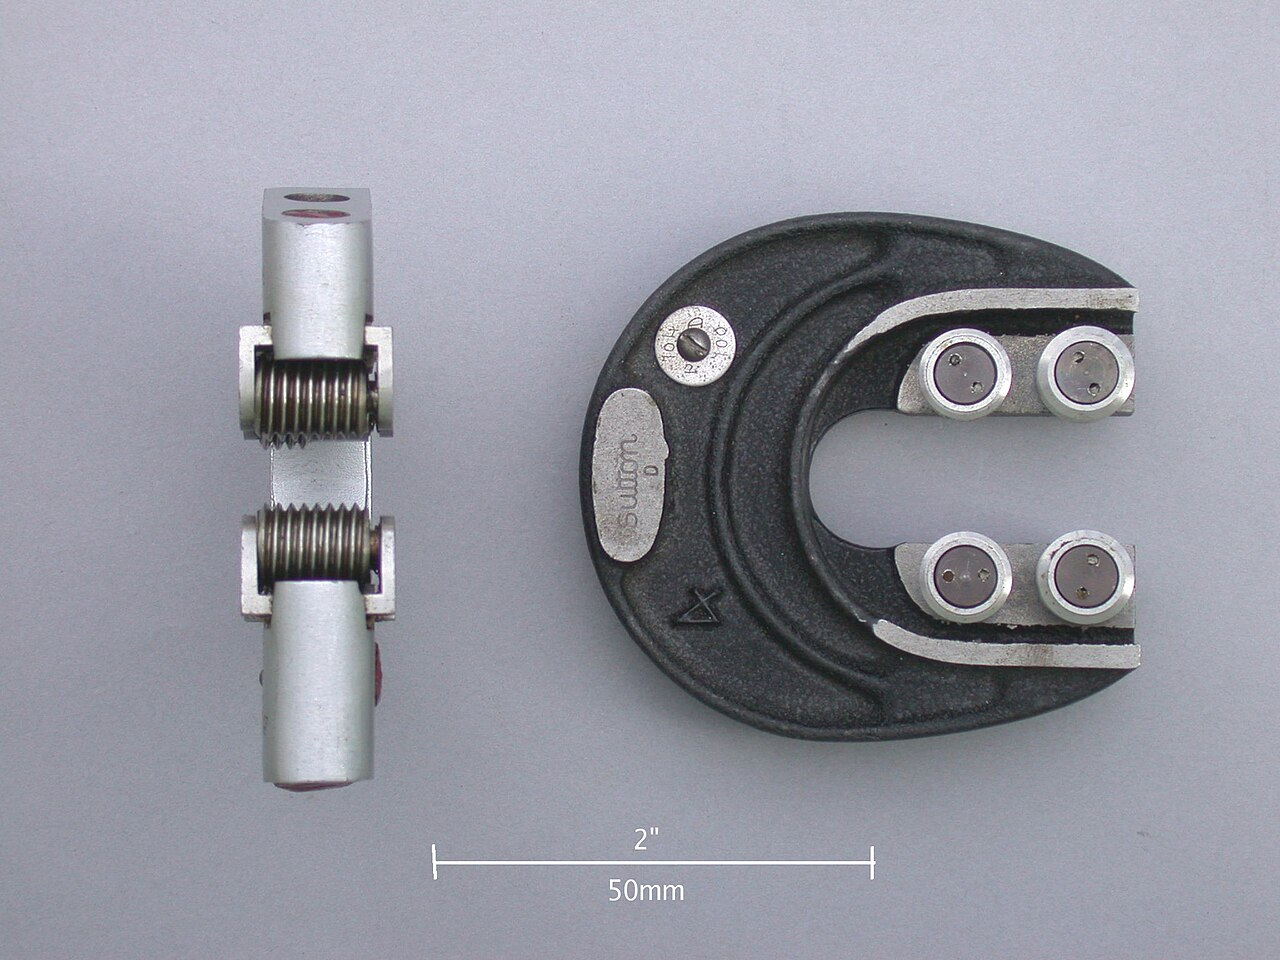
\includegraphics[width=\columnwidth]{GaugeGapThreadGoNoGo}
% {\footnotesize  \par}
%             \end{figure}
%         \end{column}
%     \end{columns}
% \end{frame}

% \begin{frame}
% 	\frametitle{Thread Snap Gauges}
%     \begin{columns}
%         \begin{column}{0.48\linewidth}
%             \begin{itemize}[<+- | alert@+>]
%                 \item Screw slid from front (go) jaws to rear (no-go) jaws
%                 \item Should freely pass go jaw, bind on no-go jaws
%             \end{itemize}
%         \end{column}
%         \begin{column}{0.48\linewidth}
%             \begin{figure}
%                 \centering
%                 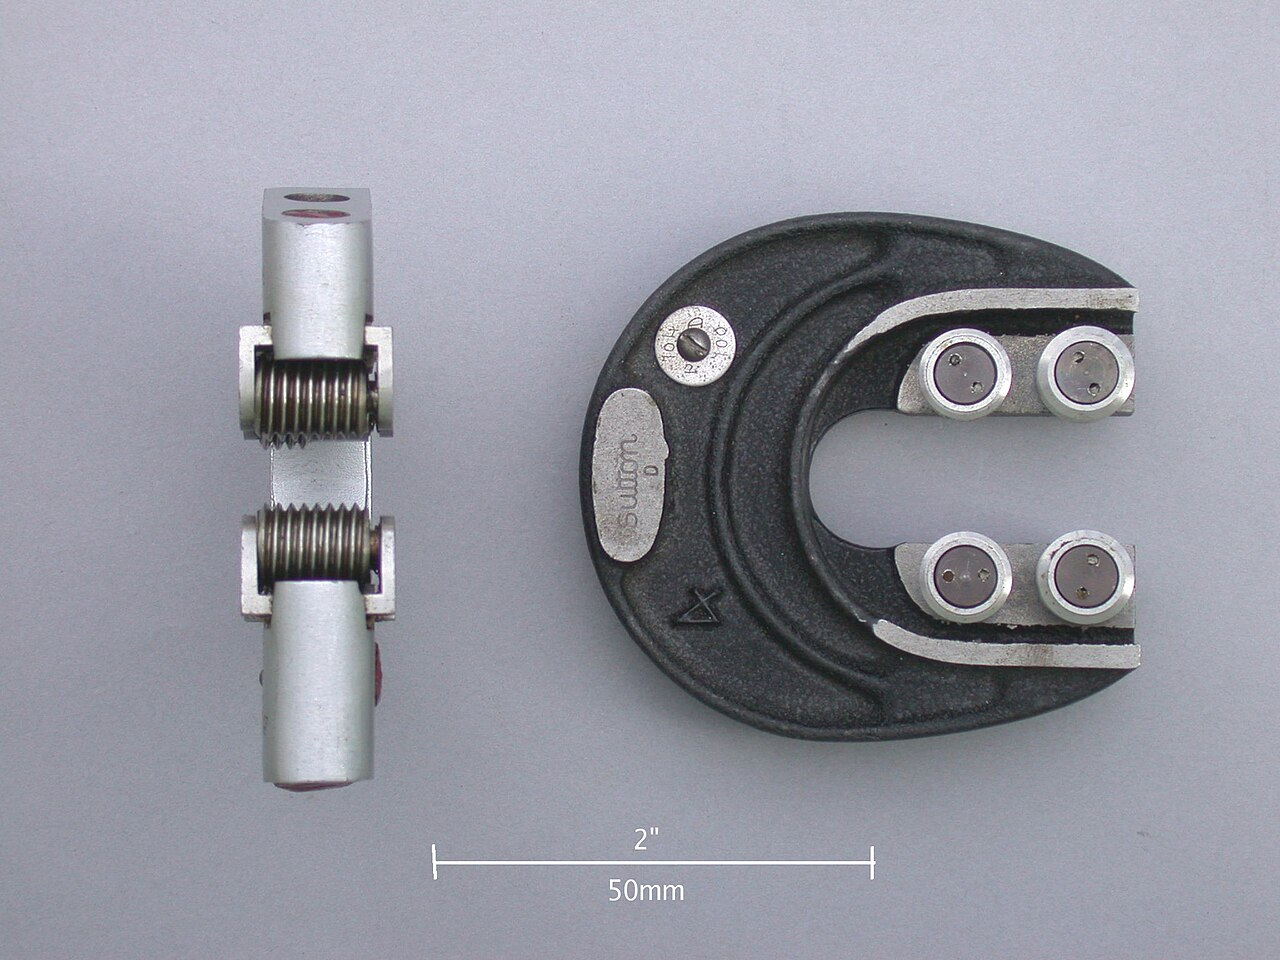
\includegraphics[width=\columnwidth]{GaugeGapThreadGoNoGo}
% {\footnotesize  \par}
%             \end{figure}
%         \end{column}
%     \end{columns}
% \end{frame}

% \begin{frame}
% 	\frametitle{Thread Pitch Gauges}
%     \begin{columns}
%         \begin{column}{0.48\linewidth}
%             \begin{itemize}[<+- | alert@+>]
%                 \item Measure thread profile only
%                 \item Really, can only reliably measure pitch
%                 \item May catch gross angle problems
%             \end{itemize}
%         \end{column}
%         \begin{column}{0.48\linewidth}
%             \begin{figure}
%                 \centering
%                 \includegraphics[width=0.5\columnwidth]{244px-Gewindeschablone}
% {\footnotesize  \par}
%             \end{figure}
%         \end{column}
%     \end{columns}
% \end{frame}

% \begin{frame}
% 	\frametitle{Thread Pitch Gauges}
%     \begin{figure}
%         \centering
%         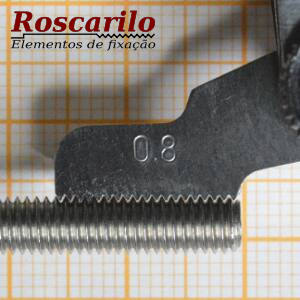
\includegraphics[width=0.5\linewidth]{080cal}
% {\footnotesize  \par}
%     \end{figure}
% \end{frame}

\begin{frame}
    \centering
    {\Huge \textbf{\textcolor{BakerADARed}{Questions?}}}
\end{frame}

\begin{frame}
    \frametitle{Copyright Notice}

    % \begin{figure}
    %     \centering
    %     
\includegraphics[width=0.25\linewidth, alt={Creative Commons Attribution NonCommercial ShareAlike logo displaying four circular icons arranged horizontally over a black banner. From left to right, the icons feature the CC logo, a person pictogram for Attribution labeled BY below, a slashed dollar sign for NonCommercial labeled NC below, and a counterclockwise circular arrow for ShareAlike labeled SA below.}]{by-nc-sa.png}
    % \end{figure}
    
    {\footnotesize
    \PresTitle \textcopyright 2026 by Brad Peirson is licensed under Creative Commons Attribution-NonCommercial-ShareAlike 4.0 International (CC BY-NC-SA 4.0). To view a copy of the official license, visit \href{https://creativecommons.org/licenses/by-nc-sa/4.0/}{https://creativecommons.org/licenses/by-nc-sa/4.0/}.

    \vspace{0.5em}

    \textbf{Exceptions and Exclusions}

    \begin{itemize}
        \item[Baker College Branding \& Trademarks:]All Baker College logos, trademarks, wordmarks, seals, slide design templates, and proprietary branding elements contained in these materials are \textbf{EXCLUDED} from the CC BY-NC-SA 4.0 license. All rights are reserved by Baker College. Express written permission from Baker College is required for any use, copying, or redistribution of these elements.
        \item[Third-Party Media \& Content:] Any third-party images, graphics, diagrams, or external media incorporated in these materials are included under their respective original licenses or permissions and are individually attributed at their point of use. 
        \item[Original Author Content:] All unattributed figures, diagrams, text, code snippets, and media are original works created by the author and are licensed under the CC BY-NC-SA 4.0 license.
    \end{itemize}
    \par}
\end{frame}

\end{document}

% \begin{frame}
%     \frametitle{Test Todo}

%     % Usage: \tikztodo[width]{height}{description/notes}
%     \tikztodo[0.7\textwidth]{4cm}{Convert block diagram of feedback loop}
% \end{frame}